\documentclass[%
%%%%%		PDFTex verwenden
pagesize=pdftex,
%%%%%   Language
german,
%%%%%   Paper size
a4paper,
%%%%%		Schriftgröße Standard 11
fontsize=11pt,
%%%%%   Get smaller borders and more space for writing
%%%%% ATTENTION be carefull with your binding! See scrbook manual! 
DIV=14,
%%%%%   Set the binding correction
BCOR=10mm,
%%%%%   Create smaler headlines
2.5headlines, 
%%%%%   Create small headings
headings=small, 
%%%%%   Use a titlepage
titlepage, 
%openbib,
%%%%%   Bibliography in Table of Contents with a chapter number
%bibliography=totocnumbered,
%%%%%   Bibliography in Table of Contents without a chapter number
bibliography=totoc,
%%%%%   Add the prefix "Appendix" to the apendix chapters
appendixprefix = true,
%%%%%   Use a twoside style
%%%%% ATTENTION oneside will change layout completely! Check this early!
twoside,
%open=any,
%oneside,
parskip=half,
numbers=noenddot
]{scrbook}
%%%%%%%%%%%%%%%%%%%%%%%%%%%%%%%%%%%%%%%%%%%%%%%%%%%%%%%%%%%%%
%% INCLUDE PACKAGES
%%%%%%%%%%%%%%%%%%%%%%%%%%%%%%%%%%%%%%%%%%%%%%%%%%%%%%%%%%%%%
\usepackage[ngerman, german]{babel}
\usepackage[utf8]{inputenc}
\usepackage{graphicx}
\usepackage{color}
\usepackage[autooneside,automark]{scrpage2}
\usepackage[stable, hang, flushmargin]{footmisc}
\usepackage[pdftex, pdfdisplaydoctitle=true, colorlinks, linktocpage, linkcolor=black, citecolor=black, urlcolor=black, hyperfootnotes=false]{hyperref}
\usepackage[all]{hypcap}  
\usepackage{bookmark}
\usepackage{longtable,ltcaption}
\usepackage{wrapfig}
\usepackage{textcomp}
\usepackage{xcolor}
\usepackage{listings}
\usepackage{enumitem}
\usepackage{subfigure}
\usepackage{fancybox}
\usepackage{tabularx}
\usepackage[T1]{fontenc}
\usepackage{caption}
\usepackage{colortbl}
\usepackage{amssymb}
\usepackage{todonotes}
\usepackage[ngerman]{translator}
\usepackage[xindy,toc]{glossaries}
\usepackage[section]{placeins}
\usepackage{scala}
\usepackage{capt-of}
\usepackage{setspace}
\usepackage{nameref}
%%%%%%%%%%%%%%%%%%%%%%%%%%%%%%%%%%%%%%%%%%%%%%%%%%%%%%%%%%%%%
%% DOCUMENT DEFINITIONS
%%%%%%%%%%%%%%%%%%%%%%%%%%%%%%%%%%%%%%%%%%%%%%%%%%%%%%%%%%%%%
\newcommand{\docAuthor}{Tom Bocklisch}
\newcommand{\docAuthorMail}{tom.bocklisch@student.hpi.uni-potsdam.de}
\newcommand{\docTitle}{Eine Architektur für ein ereignisgesteuertes, webbasiertes Backend für Project-Zoom}
\newcommand{\docTitleEng}{An eventdriven webbased backend architecture for Project-Zoom}
\newcommand{\docSupervisited}{Prof. Dr. Holger Giese, \\Thomas Beyhl, M.Sc. und\\ Gregor Berg, M.Sc.}
\newcommand{\docCity}{Potsdam}
\newcommand{\docDate}{\today}
\newcommand{\docChair}{Systemanalyse und Modellierung}%System Analysis and Modeling Group}
\newcommand{\tete}[1]{\textit{#1}}
\newcommand{\qc}[1]{\begin{sc}#1\end{sc}}
%%%%%%%%%%%%%%%%%%%%%%%%%%%%%%%%%%%%%%%%%%%%%%%%%%%%%%%%%%%%%
%% END OF DOKUMENT DEFINITIONS
%%%%%%%%%%%%%%%%%%%%%%%%%%%%%%%%%%%%%%%%%%%%%%%%%%%%%%%%%%%%%
\captionsetup{format=plain,labelfont=bf,labelsep=endash,justification=RaggedRight}%,indention=1cm}
%globale Wörtertrennung
\hyphenation{Graph-struk-tur Story-patterns Story-pattern}

\newcommand{\appendixChapter}[1]{\chapter{#1}\setcounter{page}{1}}

\def\TReg{\textsuperscript{\textregistered}}

%\zitat{quotation}
\newcommand{\zitat}[1]{
 \begin{quote}
  \fboxsep5mm
  \shadowbox{
  \begin{minipage}{0.8\textwidth}
    #1
  \end{minipage}}
\end{quote}}

%\begriff{caption}{quotation or definition}
\newcommand{\begriff}[2]{
  \begin{quote}
  \fboxsep5mm
  \shadowbox{
  \begin{minipage}{0.8\textwidth}
   \begin{center}\textbf{#1}\end{center}
   \bigskip
   #2
  \end{minipage}}
  \end{quote}}

\definecolor{lightblue}{rgb}{0.9,0.9,0.9}
\definecolor{darkred}{rgb}{0.5,0,0}
\definecolor{darkgreen}{rgb}{0,0.5,0}
\definecolor{darkgrey}{rgb}{0.8,0.8,0.8}

\renewcommand*\lstlistingname{Quelltext}
%\JavaStyleBegin{title}{caption}{label}
\newcommand{\JavaStyleBegin}[3]{
  \begin{lstlisting}[language = Java,
   frame=none,
   framerule=1pt,
   tabsize=4,
   title={#1},
   caption={#2},
   label=#3,
   backgroundcolor=\color{lightblue},
   columns=fixed,
   basicstyle=\scriptsize \ttfamily \color{black},
   commentstyle=\itshape\color{darkgreen},
   keywordstyle=\bfseries\color{blue},
   stringstyle=\color{darkred},
   showspaces=false,
   breaklines=true,
   numbers=left,
   numberstyle=\tiny \color{magenta},
   showstringspaces=false,
   captionpos=b,
   xleftmargin=0.04\textwidth, 
   morekeywords={}]}
%\end{lstlisting}
																									
\newcommand{\methode}[1]{\sl #1\normalfont}
\newcommand{\klasse}[1]{\tt #1\normalfont}
\newcommand{\attribut}[1]{\textit{#1}}
\newcommand{\interface}[1]{\tt #1\normalfont}
\newcommand{\code}[1]{\ttfamily#1\normalfont}

\newcommand{\trenn}{\left|\right|}
% Rot
\definecolor{hpired}{rgb}{0.686,0,0.204}
% Orange
\definecolor{hpiorange}{rgb}{0.867,0.380,0.031}	
% Gelb
\definecolor{hpiyellow}{rgb}{0.965,0.659,0}			%100 
\colorlet{hpiyellow2}{hpiyellow!60!white}				% 60
\colorlet{hpiyellow3}{hpiyellow!40!white}				% 40
\colorlet{hpiyellow4}{hpiyellow!20!white}				% 20
% Grau
\definecolor{hpigray}{rgb}{0.376,0.408,0.420}		%100
\colorlet{hpigray2}{hpigray!70!white}						% 70
\colorlet{hpigray3}{hpigray!50!white}						% 50
\colorlet{hpigray4}{hpigray!20!white}						% 20
% Blau
\definecolor{hpiblue}{rgb}{0,0.478,0.620}				%100
\colorlet{hpiblue2}{hpiblue!60!white}						% 60
\colorlet{hpiblue3}{hpiblue!40!white}						% 40
\colorlet{hpiblue4}{hpiblue!15!white}						% 15
%%%%%%%%%%%%%%%%%%%%%%%%%%%%%%%%%%%%%%%%%%%%%%%%%%%%%%%%%%%%%
%% PAGESTYLE SELECTION
%%%%%%%%%%%%%%%%%%%%%%%%%%%%%%%%%%%%%%%%%%%%%%%%%%%%%%%%%%%%%
\let\cleardoublepage\clearpage
\pagestyle{scrheadings}
\renewcommand*{\chapterpagestyle}{scrheadings}
\renewcommand*{\indexpagestyle}{scrheadings}
\automark[chapter]{chapter}
\clearscrheadfoot
\lehead[]{\headmark}%\parbox[b][1.3cm]{.75\textwidth}{\headmark\vskip.15cm}}
\rohead[]{\headmark}%\parbox[b][1.3cm]{.75\textwidth}{\begin{flushright}\vskip.15cm\headmark\end{flushright}}}
\cfoot{\parbox[t][1em]{\textwidth}{\centering\vfill\textbf{--} \pagemark\textbf{ --}}}
%%%%%%%%%%%%%%%%%%%%%%%%%%%%%%%%%%%%%%%%%%%%%%%%%%%%%%%%%%%%%
%% END OF PAGESTYLE SELECTION
%%%%%%%%%%%%%%%%%%%%%%%%%%%%%%%%%%%%%%%%%%%%%%%%%%%%%%%%%%%%%
\lstset{
  basicstyle=\ttfamily \color{black},
  commentstyle=\itshape\color{darkgreen},
  keywordstyle=\bfseries\color{blue},
  stringstyle=\color{darkred},
	columns=fixed
}
%%%%%%%%%%%%%%%%%%%%%%%%%%%%%%%%%%%%%%%%%%%%%%%%%%%%%%%%%%%%%
%% colored head- and footlines
\setheadsepline{1.0pt}[\color{hpired}] \setfootsepline{1.0pt}[\color{hpired}]
\setstretch{1.3}
\setcounter{tocdepth}{1}
%%%%%%%%%%%%%%%%%%%%%%%%%%%%%%%%%%%%%%%%%%%%%%%%%%%%%%%%%%%%%
\pdfminorversion=6
%%%%%%%%%%%%%%%%%%%%%%%%%%%%%%%%%%%%%%%%%%%%%%%%%%%%%%%%%%%%%
%% Glossary
%%%%%%%%%%%%%%%%%%%%%%%%%%%%%%%%%%%%%%%%%%%%%%%%%%%%%%%%%%%%%
\makeglossaries
\glossarystyle{index}
\loadglsentries{src/glossary}

%%%%%%%%%%%%%%%%%%%%%%%%%%%%%%%%%%%%%%%%%%%%%%%%%%%%%%%%%%%%%
%% Hypernationfixes
%%%%%%%%%%%%%%%%%%%%%%%%%%%%%%%%%%%%%%%%%%%%%%%%%%%%%%%%%%%%%
\hyphenation{da-ten-bank-trei-ber}

%%%%%%%%%%%%%%%%%%%%%%%%%%%%%%%%%%%%%%%%%%%%%%%%%%%%%%%%%%%%%
%% DOKUMENT
%%%%%%%%%%%%%%%%%%%%%%%%%%%%%%%%%%%%%%%%%%%%%%%%%%%%%%%%%%%%%
\begin{document}
	\selectlanguage{ngerman}

	%%% PATHES FOR GRAPHIC-FILES
	\graphicspath{{./}{img/}}
	
	%%% PDF-DOCUMENT-INFO
	\hypersetup{%
		pdftitle	= {\docTitle},
		pdfsubject	= {Bachelor's Thesis},
		pdfauthor	= {\docAuthor},
		pdfcreator	= {PDFLaTeX},
		pdfproducer	= {LaTeX with hyperref and thumbpdf}		
	}
	
	\pagenumbering{Roman}
	
	%%%%%%%%%%%%%%%%%%%%%%%%%%%%%%%%%%%%%%%%%%%%%%%%%%%%%%%%%%%%%
	%% TITLEPAGE, THANKS, ABSTRACT
	%%%%%%%%%%%%%%%%%%%%%%%%%%%%%%%%%%%%%%%%%%%%%%%%%%%%%%%%%%%%%
	%!TEX root = ../Bachelorarbeit.tex
\begin{titlepage}

\centering
\sffamily


\includegraphics[height=20ex]{logo_uni_potsdam}
\hspace{2.5cm}

\includegraphics[width=35ex]{hpi_logo_v2}
\vspace*{0.75cm}

\textsf{\Large Hasso-Plattner-Institut f\"ur IT-Systems Engineering}\\

\vspace{2cm}

\huge
\textbf{Bachelorarbeit}\\[0.4\baselineskip]
\huge
\textbf{\docTitle}\\[\baselineskip]
%\LARGE
%\textbf{Bachelorthesis}\\[0.2\baselineskip]
\Large 
\textbf{\docTitleEng}\\[\baselineskip]
\Large
\docAuthor\\[0.5\baselineskip]
{\normalsize \docAuthorMail}\\

\vfill

\large
Betreut von \docSupervisited
\\[1.0\baselineskip]
\docChair

\vspace{1cm}
\textsf{\docCity{}, \docDate}\\ %%Date - better you write it yourself.
\end{titlepage}

	\thispagestyle{empty}
	\cleardoublepage
	%$\section*{Danksagung}

Ich bedanke mich ...
	%!TEX root = ../Bachelorarbeit.tex
\addchap*{Zusammenfassung}

Im Verlauf der kreativen Design Prozesse in der HPI School of Design Thinking (D-School) entstehen eine Menge an Dokumentationsartefakten. Diese Daten sind jedoch meist in Quellen abgelegt, deren gesicherte Persistenz nur für einen beschränkten Zeitraum gegeben ist. Die Informationen aus den Wissensquellen gilt es dauerhaft zu sichern,  organisieren und für Außenstehende verständlich darzustellen. Durch die graphische Darstellung des Prozesses der Ideenfindung können sowohl die Teilnehmer eines Design Thinking-Teams selbst, als auch deren Mentoren wichtige Erkenntnisse für den weiteren Erfolg einer Idee gewinnen. Neben diesem Überblick über die Entwicklung in einem Projekt, fehlt der D-School eine Gesamtübersicht über all ihre Projekte. Diese Hilft, Abhängigkeiten der Projekte voneinander zu verdeutlichen und erleichtert die Akquirierung neuer Projekt-Themen. 

In dieser Bachelorarbeit soll das Backend der entwickelten Lösung \tete{Project-Zoom} näher erläutert werden. Die Architektur dieses Systems wird betrachtet und die zugrundeliegenden Entscheidungen erklärt. Dazu werden zu Beginn die Anforderungen des Projektpartners aufgezeigt und im Verlauf der Arbeit als Entscheidungsgrundlage verwendet. Das Backend der umgesetzten Anwendung basiert auf einer asynchronen Webarchitektur. Es wird das Konzept des Data-centric Designs umgesetzt und mit verschiedenen alternativen Konzepten im Bereich der Datenbankanbindung verglichen. Die Datenmodellierung setzt die Anforderungen der School of Design Thinking um und verwendet dabei unter anderem Datenversionierung und Datenzugriffsschutz auf Datenmodell-Ebene. Zur Anbindung von externen Komponenten und Systemen wurde ein Eventsystem umgesetzt, welches die Anpassung der Anwendung an zukünftige Bedürfnisse der School of Design Thinking erlaubt. Den Abschluss der Arbeit bildet eine Evaluierung der Anforderungen sowie ein Ausblick auf mögliche Erweiterungen.

	
	%%%%%%%%%%%%%%%%%%%%%%%%%%%%%%%%%%%%%%%%%%%%%%%%%%%%%%%%%%%%%
	%% TABLE OF CONTENT
	%%%%%%%%%%%%%%%%%%%%%%%%%%%%%%%%%%%%%%%%%%%%%%%%%%%%%%%%%%%%%
	\clearpage
	\pdfbookmark[0]{Inhaltsverzeichnis}{toc}	
	\tableofcontents
 	
 	\clearpage
	\pagenumbering{arabic}
	
	%%%%%%%%%%%%%%%%%%%%%%%%%%%%%%%%%%%%%%%%%%%%%%%%%%%%%%%%%%%%%
	%% START CONTENT
	%%%%%%%%%%%%%%%%%%%%%%%%%%%%%%%%%%%%%%%%%%%%%%%%%%%%%%%%%%%%%
	%keine Einrückung des Absatzes
	%\parindent 10pt
	%neue Zeile nach Absatz
	%\addtolength{\parskip}{\baselineskip}

	%!TEX root = ../Bachelorarbeit.tex
\chapter{Motivation}
\label{chap:Einleitung}
Die School of Design Thinking (D-School) lehrt die kreative Herangehensweise an Probleme und die Entwicklung einfallsreicher Lösungen. Die Lehre findet in verschiedenen Kursen statt. Studierenden können sich die Grundlagen im Basic-Track vermitteln lassen und anschließend bei erfolgreicher Teilnahme ihr Wissen im  Advanced-Track vertiefen. Neben diesen studentischen Kursen bietet die D-School auch Weiterbildungskurse direkt für Unternehmen an.

In solch einem Kurs wird dann in kleingruppen von ca. 6 Teilnehmern an einem Projekt gearbeitet. Das Projektthema wird dabei entweder von der D-School selbst oder vor allem bei längeren Projekten von externen Projektpartnern vorgeschlagen. 

Während der Arbeit an ihren Projekten durchlaufen die Teilnehmer verschiedene Phasen, welche vom Verstehen und Beobachten des Problemfeldes über die Definition eines Standpunktes und das Finden von Ideen bis hin zu einem Prototyp und dessen Tests reichen. Während dieser verschiedenen Phasen fallen unterschiedlichste Dokumente an, welche die Lösungsfindung dokumentieren.

Im Verlauf des Projektverlaufes kommt es durchaus vor, dass ein Team eine Phase mehrmals durchläuft oder in eine vorherige Phase zurückspringt. Dies erschwert die Organisation der Dokumente, z.B. in einer einfachen hierarchischen Struktur. Weiterhin ist es schwierig allein aus den Dokumenten deren Entstehungsreihenfolge und Bedeutung zu erfassen. Meist entstehen während eines 3 Monate andauernden Projektes verschiedenste Präsentationen, Zusammenfassungen, Prototypen, Bilder von Whiteboards und Interviewdokumentationen. Diese werden meist in der von den Studierenden bevorzugten Art und Weise gespeichert und verwaltet, z.B. mit Hilfe von Dropbox, Google Docs oder Box.

Das Verständnis der Dokumentation ist sowohl für das Projekt selbst zum verstehen und erlernen des Prozesses, als auch als Ideenquelle für zukünftige Projekte wichtig. Ferner sind die erstellten Artefakte nützlich zum Werben um neue Projektpartner, welche die Projekte betreuen. 


\section{Zielsetzung von Project-Zoom}
Project-Zoom soll der Verbesserung der Dokumentation dienen. Dazu sollen die von den Studierenden erzeugten Artefakte durch manuelles Anordnen in eine Form gebracht werden, welche den Prozess der Gruppe visualisiert. Die Mitarbeiter der D-School kann anschließend diese entstandenen Graphen nutzen um die Projektverläufe zu analysieren und gegebenenfalls den D-School Prozess anpassen.

Für eine reibungslose Integration des Systems ist vor allem die Anbindung an bereits existierende IT-Systeme und die von den Studierenden für das Projekt verwendete Software wichtig. Die Software muss dabei mit moderatem Aufwand angepasst werden können, um andere externe Dienste anbinden zu können.

\section{Abgrenzung}
Die Arbeit beschreibt und bezieht sich auf das Bachelorprojekt „From Creative Ideas to Well-Founded Engineering“ und das umgesetzte Softwaresystem Project-Zoom. An diesem Projekt haben 6 Studierenden gearbeitet und beschreiben in ihren Bachelorarbeiten das Projekt aus verschiedenen Blickwinkeln mit verschiedenen Schwerpunkten.

Tom Herolds Arbeit \cite{bp-tomh} behandelt die Interaktion mit kontextsensitiven Graphen. Es gilt die Interaktion des Studierenden mit der Nutzeroberfläche so intuitiv wie möglich zu gestallten und den Nutzer bei der Erfassung dokumentationsrelevanter Eigenschaften zu unterstützen.

Die Ausführungen von Anita Diekhoff \cite{bp-anita}  beschäftigen sich mit der ...

Norman Rzepka’s Bachelorarbeit \cite{bp-norman} thematisiert die webbasierte eventgesteuerte clientseitige Architektur von Project-Zoom. Hier wird näher darauf eingegangen, wie die Daten von der DB, über das Backend asynchron an den Client ausgeliefert werden.

Die Bachelorarbeit von Dominic Bräunlein \cite{bp-dome} erläutert das generieren und bereitstellen von semantischen Thumbnails, um dem Nutzer das Erkennen der Dokumente seines Projektes zu erleichtern und somit selbst bei wenig verfügbarem Platz so viele Informationen eines Dokumentes anzeigen zu können. 

Thomas Werkmeister befasst sich in seiner Arbeit \cite{bp-tewe} mit der Anbindung externer Systeme zur Integration von Daten. Diese aggregierte Datenbasis ist die Grundlage für die Wissensbasis und die einzelnen Projekte.

Die Komponenten die in den Arbeiten \cite{bp-tewe} und \cite{bp-dome} beschrieben sind, sind mit dem hier erläuterten Systemteil mittels eines Eventsystems verbunden. Das Client-Frontend ist über eine REST Anbindung an das Server-Backend angeschlossen. Mit der clientseitigen Implementierung der REST Schnittstelle beschäftigt sich \cite{bp-norman}.

\section{Gliederung}
In dieser Arbeit wird zuerst ein Überblick über das Gesamtsystem gegeben. Dazu werden die Anforderungen der D-School an das Backend analysiert und dienen als Grundlage für die Begründung der Verwendeten Technologien. Anschließend wird die Architektur des Backends näher erläutert. Hier liegt der Hauptfokus zunächst auf einer neuen Art und Weise eine Datenbank an eine Webapplikation anzubinden. Dann werden einige Feinheiten und interessante Stellen der Datenmodellierung von Project-Zoom beleuchtet. Den Abschluss bildet die Architektur technische Grundlage für die Anbindung externer Systeme für die Erweiterung des Systems.

%\zitat{"`Ein Zitat kann manchmal helfen ;-)"' (\cite{TODO})} 

	%!TEX root = ../Bachelorarbeit.tex
\chapter{Konzeptioneller Aufbau des Backends}

In diesem Kapitel wird die Architektur von Project-Zoom betrachtet. Begonnen wird mit einem Überblick über den Anwendungsaufbau. Anschließend wird ein konkretes Datenmodell entworfen, um daraufhin mit dem data-centric Design ein Konzept zur Umsetzung dieses Modells zu verdeutlichen.  Den Abschluss bildet ein weiterer Teil der Architektur, das Eventsystem.
%--------------------------------------------------------------------------------------------------------------------------------------------

\section{Anwendungsart}
\subsection{Webanwendung vs. native Applikation}
Eine der grundlegenden Entscheidungen in der Entwicklung ist die Art der Anwendung, für dieses Projekt kommen eine Webanwendung oder eine native Anwendung in Frage. 

Auf Grund der Anforderung der D-School, dass die Anwendung auch außerhalb der Gebäude der D-School verwendbar sein muss (vgl. REQXXX), liegt eine Webanwendung nahe. Hinzu kommt, dass die Projekt-Mitglieder bereits mit dem Umgang von Webseiten und deren Navigation vertraut sind. Für die Erweiterbarkeit stellt dies ebenfalls einen enormen Vorteil dar, da ein zentrales System gewartet werden kann und neue Funktionen einfach eingespielt werden können. Zudem dreht sich das Projekt um das Thema Dokumentation, bei der oft dazu geneigt wird, sie aufzuschieben. Eine Webseite senkt hier die Hemmschwelle und umgeht die Notwendigkeit einer Verteilung und Installation des Programms.

Eine Trennung der Applikation in Frontend und Backend erlaubt eine klare Funktionstrennung. Für Webapplikationen befindet sich das Backend auf Serverseite und das Frontend im Browser auf Clientseite. Die klassischen Aufgaben der beiden Teile sind:

\begin{itemize}
  \item Backend-Aufgaben:
  \begin{itemize}
    \item Sammeln und zur Verfügung stellen von Daten
    \item Kommunikation mit anderen Servern
    \item Validierung eingehender Daten vom Client
    \item Speicherung von Daten
    \item Business-Logik
  \end{itemize}

\item Frontend-Aufgaben:
  \begin{itemize}
    \item Kommunikation mit dem Backend zur Daten-Synchronisation 
\item Visualisierung der Daten
    \item Interaktion mit dem Nutzer
    \item Feedback an den Nutzer
  \end{itemize}
\end{itemize}

\subsection{Generelle Architektur von Webapplikation-Backends}

Die Grundlegende Architektur beim Bau einer Webanwendung hängt bei der Wahl eines Webframeworks vom Stil dieses Frameworks ab. Die Verwendung eines Webframeworks erlaubt die Konzentration auf die Umsetzung der Webschnittstelle und beschleunigt die Programmierung von Webanwendungen durch das forcieren von Prinzipien wie "Don't repeat yourself" (DRY) (vgl. \cite[p.~23]{pragmatic-programmer}) oder "Convention over Configuration" (vgl. \cite[p.~3]{maven}). Der Architekturstil den die meisten Frameworks verwenden ist das \tete{Model-View-Controller} (MVC)-Pattern\footnote{Aufgrund der allgemein üblichen Bezeichnung Model, View und Controller für die Teile einer MVC-Architekur werden diese anstatt der entsprechenden Begriffe Modell, Präsentation und Steuerung in dieser Arbeit verwendet.} (vgl. \cite[p.~14]{gang-of-four}). 

Das MVC Pattern dient der Abstraktion der Datenhaltung und Bussines-Logik von der Präsentation. Im Kontext einer Webanwendung ist die Rollenverteilung wie folgt:
\begin{labeling}{\textbf{Controller:}}
\item[\textbf{Model:}] Interaktion mit der Datenbank und Ausführung der Anwendungs-Logik
\item[\textbf{View:}] Generierung von verschiedenen Darstellungen für die Daten, in der Regel im HTML, JSON\footnote{JavaScript Object Notation, \url{http://tools.ietf.org/html/rfc4627}} oder XML\footnote{Extensible Markup Language, \url{http://www.w3.org/TR/REC-xml/}} Format.
\item[\textbf{Controller:}] Annahme von HTTP Anfragen und  Verarbeitung dieser zu Anweisungen an das Model. Erzeugen einer Antwort mit Hilfe eines Views auf Basis des veränderten Models.
\end{labeling}

\subsection{REST und CRUD}

Bei der Umsetzung von HTTP Schnittstellen hat sich der \tete{Representational State Transfer} (REST)-Stil etabliert. Dieser legt ein URL Schema für die Standardinteraktionen auf Ressourcen fest und verwendet dazu die verschiedenen HTTP Operationen. Diese Aktionen umfassen \tete{Create}, \tete{Read}, \tete{Update} und \tete{Delete} die als CRUD bezeichnet werden.

%--------------------------------------------------------------------------------------------------------------------------------------------

\section{Datenmodellierung}
\label{sec:model}
In diesem Abschnitt sollen die Besonderheiten der in Project-Zoom verwendeten Datenmodelle erläutert werden. An ausgewählten Modellen werden die Besonderheiten der Umsetzung erklärt.

\subsection{Überblick}

In der Abbildung \ref{fig:models} ist ein Auszug aus dem Datenmodell für Project-Zoom gegeben. Ein komplettes Datenmodell ist im Anhang in der Abbildung \ref{fig:complete-model} zu finden. Gezeigt sind die verschiedenen Daten Klassen und ihre Assoziationen. 

\begin{figure}[h]  
  \centering     
  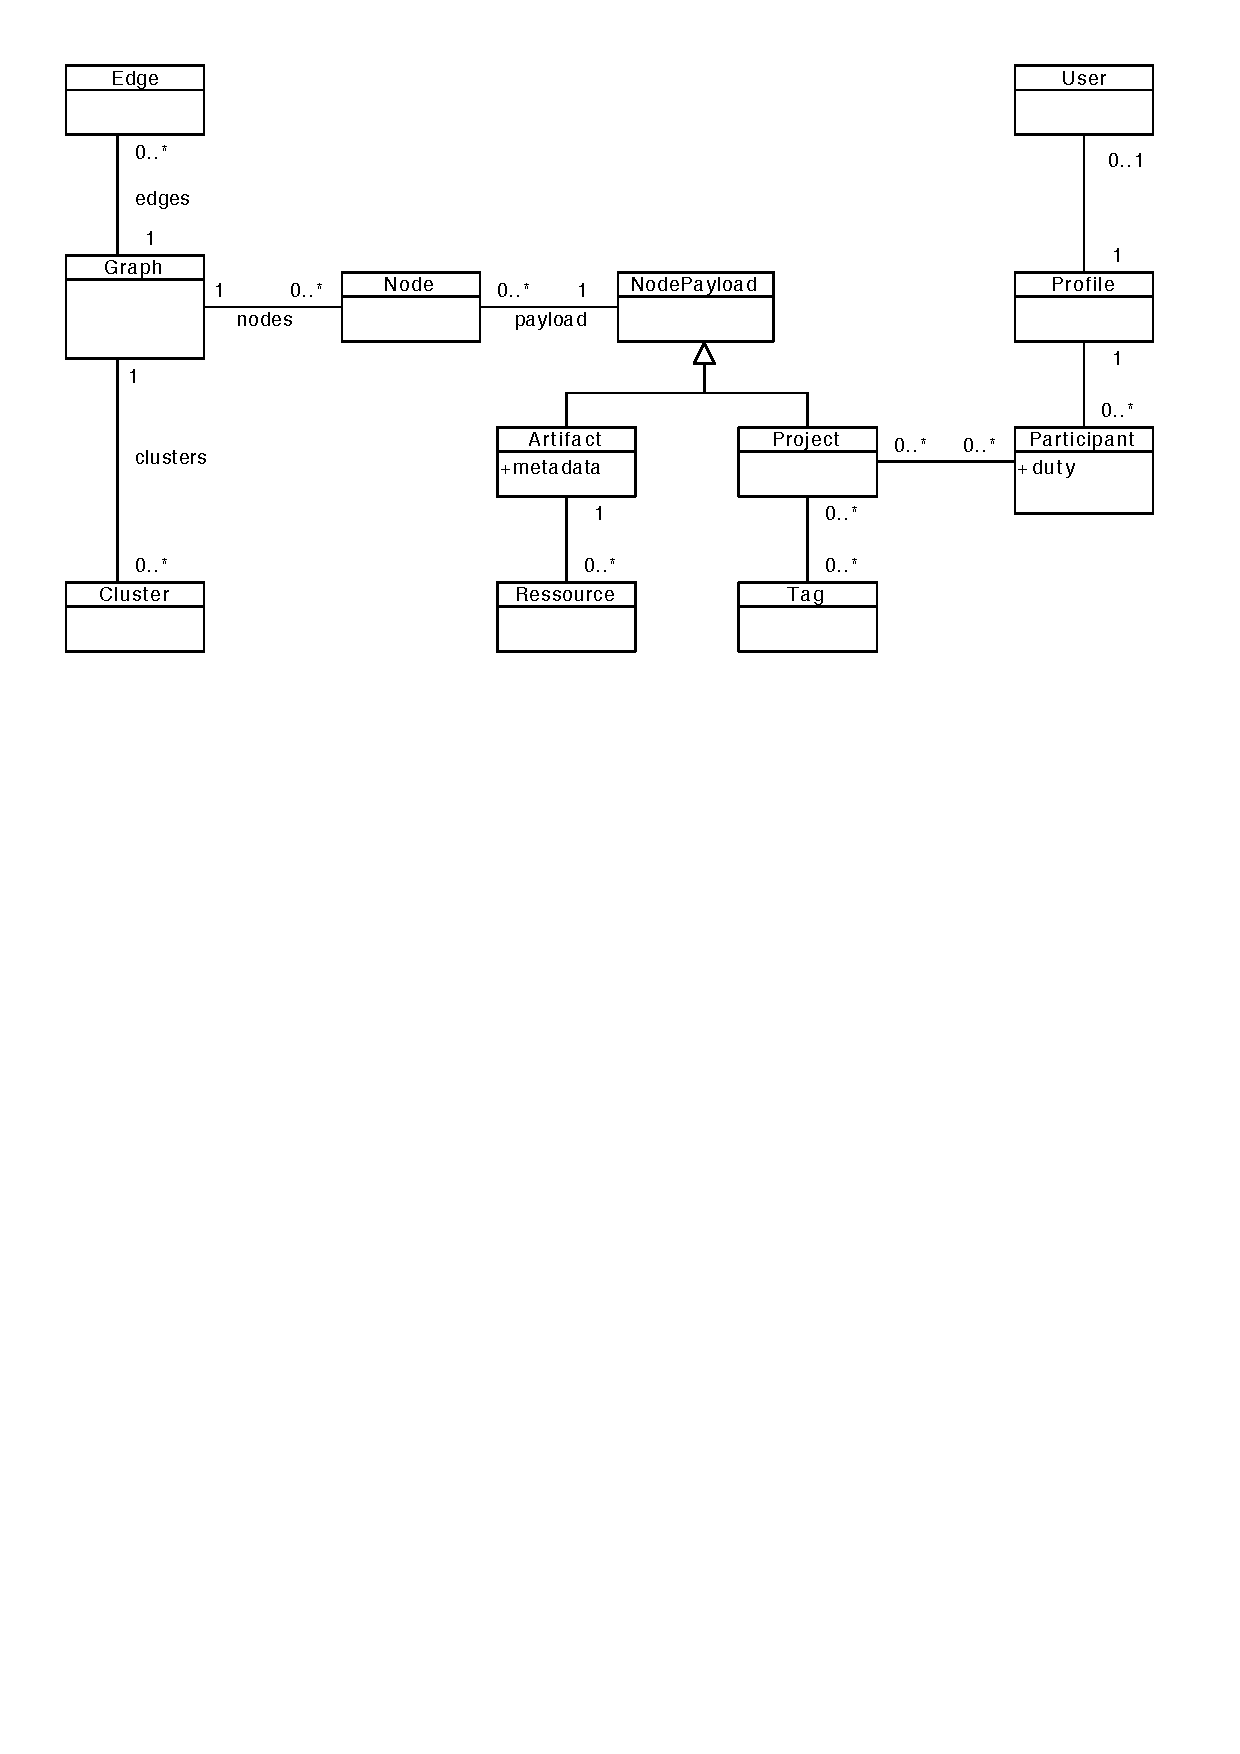
\includegraphics[width=1.0\textwidth]{img/models.pdf}  
   \caption{Ausgewählte Datenmodelle und ihre Assoziationen}
  \label{fig:models} 
\end{figure}

\subsection{Datenmodell für Graphen}
Ein Graph wurde als gerichteter Graph mit jeweils einer Liste für Knoten, Kanten und Cluster modelliert. Knoten und Kanten entsprechen denen aus der Graphentheorie bekannten Strukturen\footnote{Als konzeptionelle Referenz dient \cite[p.~531]{corman}}.  Cluster wurden eingeführt, um Nutzern die Möglichkeit zu geben, Knoten zu gruppieren und \tete{Tags} hinzuzufügen.

In der Datenbank sind für den \tete{Payload} eines Knotens nur Referenzen abgelegt. Der Payload beschreibt dabei den eigentlichen Inhalt eines Knotens, z.B. ein Projekt oder ein Artefakt. Wenn der Graph über die REST-Schnittstelle ausgeliefert wird, dann wird diese Payload-Referenz mit dem eigentlichen Inhalt des Knotens ersetzt. Dies verringert den Speicherbedarf des Graphs und verhindert das mehrfache Speichern des Payloads in der Datenbank.

\subsubsection{Versionierung}

Um die Veränderungen an einem Graph nachverfolgen zu können, wurde eine Versionierung für Graphen eingeführt. Dadurch, dass nur Referenzen auf den Inhalt eines Knotens gespeichert werden, ist die Größe eines Graphens vergleichsweise gering. Aus diesem Grund ist es möglich, alle Versionen eines Graphens in der Datenbank abzulegen. Zur Identifizierung bekommt ein Graph eine Gruppe (\tete{group}) zugewiesen. In einer Gruppe liegen die verschiedenen Versionen eines Graphen. Zusammen mit der Versionsnummer \tete{version}, welche bei jedem Update inkrementiert wird, bildet die Gruppe einen Schlüssel.

\subsubsection{Updaten eines Graphen}

Um ein Graphen-Update ausführen zu können, wurde die JSON Patch-Spezifikation\footnote{JavaScript Object Notation Patch \url{http://tools.ietf.org/html/rfc6902}} zur Veränderung von JSON-Objekten gewählt. Diese definiert eine JSON-Struktur, um ein gegebenes Objekt durch die Anwendung einer geordneten Folge von Änderungen in einen neuen Zustand zu überführen. Das Patch-Objekt ist ein JSON-Array, dessen Elemente als Operationen auf das zu verändernde JSON-Objekt angewendet werden sollen. Die definierten Operationen sind das Hinzufügen, Testen, Entfernen, Ersetzen, Verschieben und Kopieren von Attributen.

Alternativ bestünde die Möglichkeit, bei jeder Änderung den kompletten, geänderten Graphen zu senden. Da es sich hier um kleine Objekte handelt, wäre der Mehrbedarf an Bandbreite vertretbar. Für den Mehrnutzerbetrieb ist allerdings die Verwendung von JSON-Patch vorteilhaft, denn durch das explizite Senden der Änderungen ist ein Zusammenführen gleichzeitiger Änderungen von unterschiedlichen Quellen einfacher. Im Hinblick auf ebendiesen Vorteil wurde in Project-Zoom JSON-Patch verwendet. Die Implementierung im Frontend ist in \cite{bp-norman} näher beschrieben.

\subsection{Datenmodell für Artefakte}

\tete{Artefakte} werden durch externe Konnektoren gefunden und anschließend durch den Backend-Core in der Datenbank abgelegt, wo alle Informationen enthalten sind, die charakteristisch für das jeweilige Artefakt sind. Eine Besonderheit zeigt sich im Feld \tete{metadata}. Hier können alle Informationen eines Connetors gespeichert werden, die keinem allgemeinen Feld zugeordnet werden können. Durch diese Speicherung von Informationen, die zwar im Moment für die Anwendung irrelevant sind und die nicht von allen Connectoren geliefert werden können, vermeidet man einen Informationsverlust. Bei der Weiterentwicklung der Anwendung können dann Informationen aus diesen Metadaten extrahiert und als eigenständige Felder verwendet werden. 

Zu einem Artefakt sind verschiedene \tete{Ressourcen} abgelegt. Eine Ressource bezieht sich hierbei auf die digitale Repräsentation eines Artefakts. Das heißt, dass es zu jedem Ressourcenobjekt in der Datenbank eine zugehörige Datei im Dateisystem gibt. Beispielsweise ist die Originale Datei eine Ressource, generierte Thumbnails sind weitere. Das Feld \tete{typ} beschreibt die Art der Ressource und erlaubt einem Client die differenzierte Behandlung unterschiedlicher Typen.  

\subsection{Datenmodell für Nutzer}

Neben Artefakten können durch einen externen Connector auch Profile gesammelt werden. Diese Profile bestimmen die Zugriffsrechte eines Nutzers. Der mit einem Profil verknüpfte User enthält die Anmeldeinformationen, welche für die Authentifizierung benötigt werden. Ein User wird erst dann an ein Profil angehangen, wenn sich ein Nutzer mit der im Profil angegebenen E-Mail-Adresse für Project-Zoom registriert. Aus diesem Grund ist es auch nur Nutzern erlaubt sich zu registrieren, für die bereits ein Profil existiert.

Die Abspaltung des Users als Container für die Authentifizierungsinformationen vom Profil hat weiterhin den Vorteil, dass diese Informationen nicht über einen Konnektor geändert werden können. Wäre das der Fall, so könnte ein Angreifer die Log-In-Informationen für Project-Zoom durch das Verändern von Daten in einem Konnektor so anpassen, dass er Zugriff auf den Nutzer Account bekommt.

%--------------------------------------------------------------------------------------------------------------------------------------------

\section{Data-centric Design}
\label{sec:dcd}
In diesem Kapitel wird die grundlegende Architektur der Anbindung eines persistenten Speichers im Core von Project-Zoom näher erläutert. Das gewählte Design hat vorrangig Auswirkungen auf die Art und Weise, wie der Code für Datenmodelle geschrieben wird, erstreckt sich aber als Betrachtungsweise über die gesamte Architektur. Zuerst wird das verwendete Data Centric Design näher beschrieben und mit alternativen etablierten Formen der Datenbankanbindung verglichen. Im Kapitel \ref{sec:umsetzung_dcd} wird näher auf die Umsetzung des Designs in Project-Zoom eingegangen

\subsection{Motivation}
\label{sec:dcdmotivation}
Das JSON Coast-To-Coast Design als Umsetzung des data-centric Designs wurde erstmals zusammenhängend und mit Beispielen unterlegt von Pascal Voitet dargestellt \cite{jctc}. Voitet ist selbst Mitwirkender am Open-Source-Projekt Play und Autor von Scala-Bibliotheken (\tete{play-reactivemongo}\footnote{\url{ https://github.com/zenexity/Play-ReactiveMongo}}, \tete{play-autosource}\footnote{\url{ https://github.com/mandubian/play-autosource}}). 

Ein Backend für eine Webapplikation ist zunehmend eine Verbindung zwischen verschiedenen anderen Backends und Frontends. Diese Entwicklung geht auf die Bereitstellung von APIs für viele große und kleine im Web verfügbare Dienste zurück. Anwendungen, welche Daten vorrangig aus anderen Quellen aggregieren, sind zum großen Teil mit der Datenmanipulation beschäftigt. Hier bietet sich ein data-centric Design an. Grundlegend für das Design sind dabei drei Entwicklungen: Zum einen das Aufstreben von NoSQL-Datenbanken und zum anderen asynchrone Datenbanktreiber mit einfachen Methoden zur JSON-Manipulation.

\subsubsection{NoSQL}
Die Entwicklung der Datenbankmanagementsysteme bestand viele Jahre lang in der Optimierung und Verbesserung bestehender relationaler Datenbankmodelle. Im Jahr 1998 kam der Term Not-only SQL (NoSQL) auf (vgl. \cite{storage-solutions}). Heute gibt es verschiedene etablierte Datenbanken, die keine reinen SQL Datenbanken mehr sind, wie beispielsweise MongoDB, Apache CouchDB und Apache Cassandra\footnote{\url{http://cassandra.apache.org}}.
\todo{Vorteil gegenüber SQL in bzug zu DCD}

\subsubsection{Datenbanktreiber}
\label{sec:reactive}
Für die Anbindung von relationalen Datenbanken gibt es in Java die Java Database Connectivity (JDBC). Diese Schnittstelle abstrahiert über Datenbanken und deren Treiber, indem eine einheitliche API angeboten wird. Ausgerichtet ist JDBC auf relationale Datenbanken \cite{reese2000database}.

Um NoSQL-Datenbanken anzubinden, benötigt man, wie bei JDBC, einen eigenen Treiber. Der Unterschied ist, dass es hier keine Abstraktionsebene über verschiedene NoSQL-Datenbanken gibt. Dies liegt vorrangig an der sich stark unterscheidenden Struktur der einzelnen Speichersysteme. Die unterschiedlichen NoSQL-Datenbanken sind jeweils speziell auf eine bestimmte Aufgabe ausgerichtet, wie z.B. auf Durchsatz, verteilte Umgebungen oder flexible Datenschemas. 

\tete{ReactiveMongo} ist ein asynchroner Datenbanktreiber für MongoDB und die Programmiersprache Scala. Die Vorteile eines asynchronen Treibers liegen auf der Hand: Für jede synchrone Datenbankabfrage wird normalerweise ein Thread verwendet, der bis zur Antwort blockiert ist. Bei mehreren Datenbankabfragen pro Request werden bei Last viele Threads benötigt, um Datenbankabfragen auszuführen. Asynchrone Treiber umgehen dieses Problem, indem sie Threads, welche Datenbankabfragen ausführen, nicht blockieren. Für dieses Konzept ist es notwendig, Platzhalter einzuführen. Diese ersetzen das Ergebnis, solange es noch nicht vorhanden ist.

\begin{lstlisting}[label=lst:asyncaccess, caption=Funktionssignatur für asynchronen Datenbankzugriff]
def findOneById(bid: BSONObjectID): Future[Option[Graph]]
\end{lstlisting}
\todo{Vorteil Asynchronität, Referenz Anforderungen}
 
Im Quelltext \ref{lst:asyncaccess} zeigt die Funktionssignatur den Rückgabetyp \tete{Future[Option[Graph]]}. \tete{Future} ist hierbei ebendieser Platzhalter für ein Ergebnis, welches noch nicht existiert. Um auf das Ergebnis eines \tete{Futures} zu reagieren, können verschiedene \tete{Callbacks} festgelegt werden.


\subsubsection{Manipulation von JSON}
Das data-centric Design basiert auf der Idee der direkten Manipulation von Daten. Für eine Umsetzung des data-centric Designs mit Hilfe von JSON benötigt man somit eine Bibliothek, welche die Möglichkeit bietet, JSON zu transformieren und zu validieren.
 
Eine solche Bibliothek, welche das Validieren, Transformieren und Serialisieren erlaubt, ist Play-JSON. Ein Beispiel, wie solch eine Transformation und Validierung aussieht, ist im Anhang im Quelltextauszug \ref{app:jsonbsp} zu sehen. Dort wird ein JSON-Objekt erzeugt, welches anschließend zuerst transformiert wird, indem das Attribut \tete{role} angehangen wird, und danach validiert wird. Bei der Validierung wird überprüft, ob der Nutzer über 18 Jahre alt ist.

\subsection{Idee hinter data-centric Design}
Das Ziel im data-centric Design ist die direkte Manipulation von Daten. Der Fokus des Designs liegt dabei sowohl auf der Datenmanipulation als auch auf dem Datenfluss. Wie bereits im Abschnitt \ref{sec:dcdmotivation} beschrieben, sind Webapplikation Backends immer häufiger Knotenpunkte in einem mehrere Server durchlaufenden Datenfluss. Ein Teil dieses Datenflusses, die Kommunikation des Backends mit der Datenbank und dem Client, ist in Abbildung \ref{fig:dataflow} dargestellt. 

\begin{figure}[h]   
  \centering     
  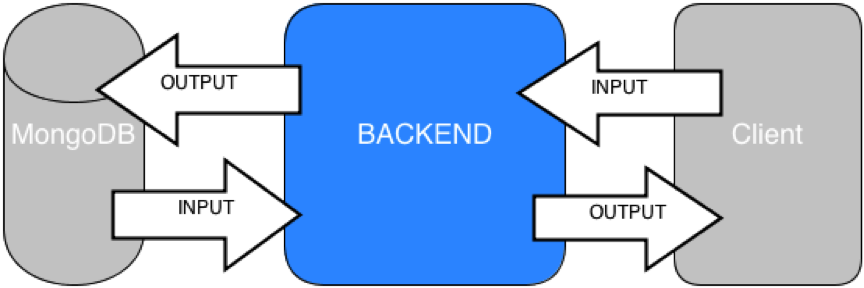
\includegraphics[width=0.8\textwidth]{img/dataflow.png}  
   \caption{Datenfluss zwischen Datenbank, Backend und Client}   
  \label{fig:dataflow} 
\end{figure}

In diesem Datenfluss soll es keine implizite Umwandlung der Daten in Objekte der Programmiersprache\footnote{Es ist bekannt, dass die Repräsentation der Daten des Datenflusses ebenfalls in Objekten der Programmiersprache erfolgt (beispielsweise JSON-Objekte). Mit dem Ausdruck ist die Überführung der Daten aus einem allgemeinen Modell (z.B. JSON) in eine spezifische Objektdarstellung (z.B. ein Objekt einer User-Klasse) gemeint.} geben. Für ein einfaches Durchleiten der Daten aus der Datenbank zum Client oder von einer anderen Webressource zum Client ist eine Umwandlung nicht notwendig oder sinnvoll. 

Im Gegensatz zu anderen Modellen ist die Abstraktion von der Datenquelle kein Ziel des data-centric Designs. Das Festlegen auf eine Datenquelle bei der Entwicklung eines Systems erlaubt die Verwendung aller Funktionen, die diese Datenquelle zur Verfügung stellt. Beispielsweise erlaubt MongoDB die Verwendung sogenannter \tete{Capped Collections}\footnote{Mehr Informationen zu Capped Collections z.B. auf \url{http://docs.mongodb.org/manual/core/capped-collections/}}, welche auf hohen Durchsatz optimiert sind. Diese verhalten sich wie eine zirkuläre Queue mit begrenzter Größe. Viele Datenbanken besitzen spezielle, stark angepasste Funktionen, auf die jedoch bei der Verwendung von allgemeinen Datenbank APIs (z.B. JDBC) meist nicht zugegriffen werden kann. Ein Nachteil dieser engen Kopplung ist, dass der Austausch der Datenquelle dadurch schwieriger ist. 

Eine Deserialisierung der Daten in Objekte ist für komplexe Business-Logik von Vorteil. Statische Datenmodelle sollten immer dann verwendet werden, wenn die Manipulation der Daten kompliziert wird oder wenn die Verwendung externer Bibliotheken eine Objektrepräsentation benötigt.  \todo{näher erläutern}

Nach Voitet ist die Frage also nicht, statische Datenmodelle zu vergessen, sondern sie nur dann zu benutzen, wenn sie notwendig sind. Einfache und dynamische Strukturen sollten so oft es geht erhalten bleiben (vgl. \cite{jctc}).

\subsection{Abgrenzung zur objektrelationalen Abbildung}
Das \tete{Object-relational Mapping} (ORM) bezeichnet man auch als \tete{All-Model-Approach}. Hierbei erfolgt die Kommunikation mit der Datenbankschnittstelle über Objekte der Programmiersprache. Abfragen an die Datenbank resultieren in Objekten der Programmiersprache. Der Fokus der objektrelationalen Abbildung liegt in der Überführung von Objekten der objektorientierten Programmierung in ein relationales, tabellenorientiertes Schema (vgl. \cite{wambler}). 

\begin{figure}[h]   
  \centering     
  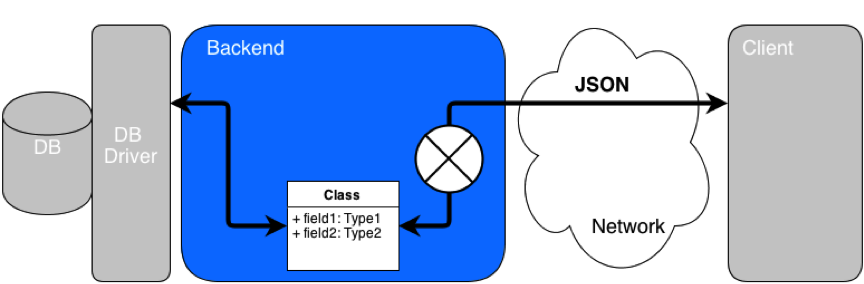
\includegraphics[width=0.8\textwidth]{img/orm.png}  
   \caption{Datenfluss einer Applikation bei Verwendung eines ORM Frameworks}   
  \label{fig:orm} 
\end{figure}

Der wichtigste Vorteil eines Frameworks für die objektrelationale Abbildung liegt in der Abstraktion von der Datenbank. Für die Business-Logik gibt es keinen Unterschied zwischen Objekten aus der Datenbank und Objekten der Programmiersprache. Die Datenbank kann meist ohne Änderungen an der Applikation ausgetauscht werden.
\todo{Abgrenzung zu NoSQL klarer}

\FloatBarrier
\subsection{Objektrelationale Unverträglichkeit}

Ein ORM bringt konzeptionelle Probleme mit sich. Diese werden in der Literatur (vgl. \cite{ireland2009classification}) in der Regel als \tete{Object-relational Impedance Mismatch} (ORIM) bezeichnet. Die objektrelationale Unverträglichkeit resultiert aus den Unterschieden im zugrundeliegenden Konzept, sowie aus Differenzen in der Darstellung und den Erwartungen des Entwicklers (vgl. \cite{bowers}).

Folgende Herausforderungen ergeben sich für die praktische Arbeit mit einem ORM:

\begin{itemize}
  \item Die Abbildung der Relationen zwischen den Objekten ist komplex. Es müssen One-to-One, One-to-Many und Many-to-Many Abhängikeiten ins relationale Schema übertragen werden.
\item Ein weiterer zentraler Punkt ist die Abbildung von Hierarchien und Vererbungen aus der objektorientierten Programmierung in das physische Datenmodell. 
\item Innerhalb des ORM muss es ein Objekt-Caching geben. Dieses ist notwendig um die Illusion zu erzeugen, dass es sich um ein Objekt der Programmiersprache handelt. Denn wird ein Objekt mehrmals aus der Datenbank abgefragt, so muss ein referenzgleiches Objekt zurückgegeben werden (vgl. \cite{inappropriate-abstractions}).
\item Der Entwickler muss die ORM-Limitierungen, die sich aus dem ORIM ergeben, akzeptieren. Die Probleme müssen somit bekannt sein, um sie bereits bei der Datenmodellierung zu umgehen (vgl. \cite{vietnam}). 
\end{itemize}

Ted Neward, Autor von „The Busy Java Developers Guide to Scala“ \cite{busy-to-scala}, macht den frühen Erfolg von objektrelationalen Abbildungen und die Erleichterungen, welche die ersten ORMs mit sich brachten, dafür verantwortlich, dass zum Teil ORMs verwendet werden, ohne deren Limitationen zu beachten. Das wiederum führt zu Mehraufwand an Zeit und Energie für die Erhaltung und Anpassung an alle Nutzungsfälle (vgl. \cite{vietnam}).

\subsubsection{Unterschiede zum data-centric Design}
Das data-centric Design ist viel stärker an die Datenbank gebunden und deren Austausch ist deutlich schwieriger. Dies sorgt dafür, dass keine Illusion einer abstrahierten Datenbank entsteht. Da das data-centric Design ein Ansatz mit funktionalem Hintergrund ist, sind die Datenstrukturen in der Regel unveränderbar.\todo{Unterschied zwischen Struktureller und Objektverränderbarkeit} Ein Caching zur Sicherung der Objektidendität ist daher nicht notwendig. Die Objektgleichheit ist in diesem Fall über Wertgleichheit definiert (vgl. Scala Case Klassen in \cite{scala-case-class}). Im Gegensatz zum ORM muss der Entwickler beim data-centric Design selbst um die Darstellung und Umwandlung seiner Daten in das Datenbankformat kümmern. Durch die Verwendung einer objekt- oder dokumentenbasierten Datenbank ist diese Umwandlung einfacher und mit weniger Problemen behaftet, als eine Konvertierung in ein relationales Schema.

\subsection{Abgrenzung zu Datenzugriffsobjekten}
Implementierungen von Datenzugriffsobjekten, in der englischsprachigen Literatur \tete{Data Access Object} (DAO) oder \tete{Data Access Procedure}, basieren auf dem \tete{Data Access Object} Pattern (vgl. \cite{j2ee-pattern}).  Das Pattern hat das Ziel, den Datenzugriff und die Datenmanipulation in einen separaten Layer auszulagern. Daraus ergibt sich eine Kapselung der Datenbankzugriffe an einem Ort der Applikation. Bei der Umsetzung gibt es die Möglichkeit, ein DAO zur Abstraktion der Datenbank als Ganzes zu verwenden oder für jede einzelne Datenbankstruktur ein DAO anzulegen.

Der Hauptfokus liegt in der Abstrahierung der Datenbank. Bei Änderungen an der Datenquelle müssen in der Regel nur die Datenzugriffsobjekte angepasst werden, denn der Anwendungscode bleibt in der Regel unberührt. Die Serialisierung der Daten von den Strukturen der Anwendung in Strukturen der Datenbank ist nicht Aufgabe des DAO, sondern des \tete{Data Transfer Object} (DTO)\footnote{vgl. J2EE Patterns – Data Transfer Object \url{http://www.oracle.com/technetwork/java/transferobject-139757.html}}.

Im DAO findet über einen Datenbanktreiber direkter Zugriff auf die Datenbank statt. Man kann das Datenzugriffsobjekt somit als Bindeglied zwischen Datenbank und Applikation sehen. Durch die direkte Kommunikation mit der Datenquelle können alle unterstützten Funktionen ausgenutzt werden. 

Sowohl DAO als auch ORM haben die Abstrahierung der Datenbank als Ziel. Im Gegensatz zum DAO geht das ORM jedoch noch einen Schritt weiter und abstrahiert nicht nur über die Funktionen, welche durch die Datenbank zur Verfügung gestellt werden, sondern auch über die Innere Struktur der Datenquelle. In der Regel bauen ORM-Implementierungen auf dem Data Access Object Pattern und dem Data Transfer Object Pattern auf.

\subsubsection{Unterschiede zum data-centric Design}
Das DAO-Pattern enthält, ähnlich dem data-centric Design, keine Serialisierung oder Deserialisierung. Beide Designs können sehr gut zusammen verwendet werden. Der Datenfluss kann so durch ein DAO realisiert werden. Dadurch wird eine deutlich stärkere Kapselung erreicht. Voitet benutzt in seinen Beispielen kein DAO, sodass sich die Datenbankabfragen über den kompletten Quellcode verteilen. Während das bei Beispielapplikationen oder kleinen Anwendungen kein Problem darstellt, geht bei größeren Anwendungen mit vielen verschiedenen Datenmodellen schnell die Übersichtlichkeit verloren. Die Verwendung eines Datenzugriffsobjektes führt zu einem \tete{Single Point of Responsibility}\footnote{ Single Responsibility Principle (SRP), vgl. \cite[p.~339]{design-patterns}}
 und stärkt somit die Struktur des gesamten Projektes. 

\subsection{Grenzen des data-centric Designs}
Das data-centric Design eignet sich sehr gut für \tete{Create-Read-Update-Delete} (CRUD)-Anwendungen. Dort liegt der Fokus auf der Datenmanipulation, was zum Grundsatz des Designs von Project-Zoom passt.

Es erfolgt eine explizite Bindung an das Datenmodell. Durch die Nähe zur Datenquelle können spezifische Fähigkeiten einer Datenquelle genutzt und Anfragen effektiver gestaltet werden. Die dynamischen Strukturen des Datenmodells ermöglichen eine leichte Veränderbarkeit des Modells sowie einfache Verknüpfungen zwischen Daten.

Grenzen sind dem data-centric Design vor allem durch die Business-Logik gesetzt. Durch die dynamischen Strukturen im Design ist der Code meist komplizierter und länger.

Ohne die Verwendung eines DAO gibt es in diesem Design keinen Single point of responsibility für Datenbankzugriffe. Das erschwert wiederum Änderungen am Schema, da diese zu unvorhergesehenen Problemen an anderen Stellen im Anwendungsquelltext führen können. Aus diesem Grund sollten bei diesem Design ein oder mehrere Datenzugriffsobjekte verwendet werden. Ein weiterer Vorteil bei der Verwendung eines DAO ist, dass die Datenquelle deutlich leichter ausgetauscht werden kann durch die Zentralisierung der Datenbankanfragen im Datenzugriffsobjekt.

%--------------------------------------------------------------------------------------------------------------------------------------------

\section{Eventsystem}
In den Anforderungen REQXXX wurde festgehalten, dass die von den Teams erstellten Dokumente aus der jeweiligen \gls{Box}\footnote{\url{http://box.com}} für die Studierenden in Project-Zoom zur Verfügung stehen. Diese Verfügbarkeit soll schnellstmöglich nach Hinzufügen einer neuen Datei zur \gls{Box} gegeben sein (vgl. REQXXX). Hierfür ist es sinnvoll ein asynchrones System zu bauen.  Neben der Anbindung von \gls{Box} ist für die Zukunft auch der Zugriff auf facebook\footnote{The Facebook, \url{http://facebook.com}}, Dropbox\footnote{Dropbox, \url{http://dropbox.com}} und Netzwerkdateisysteme\footnote{Ein Netzwerkdateisystem ist ein Dateisystem, auf welches von Rechnern im selben Netzwerk zugegriffen werden kann, um zum Beispiel Dateien zu lesen.} vorgesehen. Es zeigt sich, dass ein paralleles, unabhängiges Abfragen der einzelnen Dienste notwendig ist.

Ein Eventsystem basiert auf dem Prinzip des Abonnierens und Veröffentlichens von Nachrichten und modelliert eine Eine-zu-Viele-Relation. Ein sogenannter \tete{Publisher} sendet seine Events, welche anschließend vom \tete{Dispatcher} an die \tete{Subscriber} verteilt werden. Die Subscriber können dieses Event schließlich abarbeiten. Dabei entsteht eine Asynchronität, da der Sender beim Emittieren einer Nachricht sofort sequentiell weiterarbeiten kann und die Bearbeitung des Events nicht abwarten muss.

\begin{figure}[h]  
  \centering     
  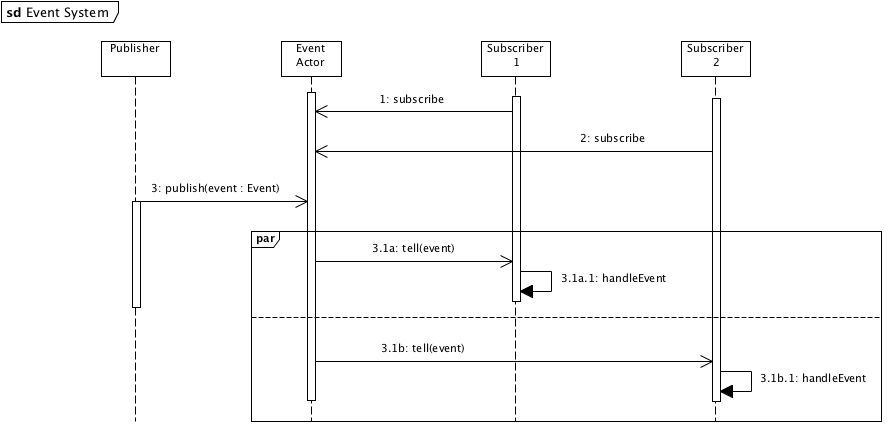
\includegraphics[width=1.0\textwidth]{img/event_system.png}  
   \caption{Funktionsweise des Eventsystems an einem Beispiel}   
  \label{fig:event-system} 
\end{figure}

Die parallele Abarbeitung von verschiedenen Aufgaben ist ein wichtiger Bestandteil von Project-Zoom. Ein Beispiel hierfür ist das Erzeugen von Thumbnails, was bei größeren Dateien eine gewisse Zeit in Anspruch nehmen kann. Diese Thumbnails werden für jedes durch einen Konnektor gefundene Artefakt erzeugt. Während der Thumbnailerzeugung muss die Webapplikation weiterhin Client-Anfragen beantworten können, weswegen die Thumbnailgenerierung ausgelagert wurde.

Ebenfalls von Bedeutung ist die Ausfallsicherheit. Der Ausfall einer einzelnen Komponente darf die Stabilität des Gesamtsystems nicht beeinträchtigen. Eine falsch konfigurierte OpenOffice-Anbindung, welche der Thumbnailgenerator benötigt (vgl. \cite{bp-dome}), darf selbst wenn der Thumnailerzeuger nicht mehr in der Lage ist zu arbeiten, das System nicht zum Stillstand bringen.

Ein weiterer Vorteil ist die Flexibilität, die durch ein Publisher-Subscriber-Modell erreicht wird. Wenn eine neue Komponente eingebunden werden soll, so kann sich diese auf bereits emittierte Nachrichten abonnieren und somit auf Ereignisse im Gesamtsystem reagieren.

In Abbildung \ref{fig:event-system} ist der Aufbau eines Eventsystems zu sehen. Der Dispatcher ist der Dreh und Angelpunkt im Eventsystem, denn er verwaltet die Abonnements und verteilt die Events an die Subsciber. Dies stellt eine Schwachstelle im Eventsystem dar, es existiert ein \tete{Single Point of Failure}. Ein Ausfall kann durch die Vervielfältigung des Dispatchers vermieden werden, wobei eine gemeinsame Datenbasis für alle Dispatcher notwendig ist. 


	%!TEX root = ../Bachelorarbeit.tex
\chapter{Umsetzung des Backends}

Die Umsetzung der gewählten Architektur und Konzepte in Project-Zoom ist Thema dieses Kapitels. Zuerst wird auf die Technologieauswahl eingegangen und die Implementierung des data-centric Designs kurz erläutert. Anschließend wird die Realisierung der Anbindung der externen Komponenten an das Eventsystem am Beispiel verdeutlicht. Den Abschluss bilden Auswertung sowie Betrachtung der Umsetzung der Anforderungen. 

\section{Technologieauswahl}

\subsection{Scala im Web: Play Framework}
Die Auswahl der Programmiersprache wurde vor allem von dem Gedanken geprägt, eine Sprache zu finden, die einerseits auf benötigte Bibliotheken zugreifen kann und andererseits eine kurze Einarbeitungszeit benötigt. Für die Arbeit mit Thumbnails hat sich die Bibliothek \tete{Apache Tika}\footnote{Apache Tika, \url{http://tika.apache.org} (Zugriff 29.06.13)} als besonders wertvoll erwiesen. Nähere Informationen zu dieser Bibliothek finden sich in \cite{bp-dome}. Da Apache Tika in Java geschrieben wurde, musste die Wahl auf eine Sprache fallen, welche in der Lage ist, Java-Bibliotheken anzusprechen. 

Um die verschiedenen Sprachen und ihr jeweiliges Webframework zu evaluieren, wurde sich mit den in Tabelle \ref{tab:FrameWorkVergleich} aufgelisteten Kombinationen näher beschäftigt. Dazu wurde von den Backend-Entwicklern jeweils eine kurze Hello-World-Anwendung aufgesetzt. Dadurch konnte festgestellt werden, ob der Arbeitsablauf, der Aufwand und der zu erzeugende Quellcode angemessen sind. Neben dieser praktischen Kurzevaluierung wurden einige Fakten zusammengetragen, um die Entscheidung zu erleichtern. Die Kriterien Asynchronität und Zustandslosigkeit sind dabei vor allem im Kontext eines asynchronen Eventsystems von Interesse. Bezüglich der Indikatoren \tete{Adoption Ready}\footnote{Umfrage von InfoQ mit 1894 Teilnehmern auf \url{http://www.infoq.com/research/jvm-web-frameworks} (Zugriff 26.06.13). Erfragt wurde eine Einschätzung der Reife des Frameworks. Der Stand bei Abruf findet sich in der Tablle \ref{fig:infoq-survey} im Anhang.} und \tete{Importance}\footnote{Entnommen aus der bereits erwähnten InfoQ-Umfrage. Erfragt wurde eine Einschätzung der Relevanz des Frameworks.} befinden sich alle Frameworks auf einem ähnlichen Niveau. 

In die nähere Auswahl kamen Java, Groovy und Scala\footnote{Nähere Informationen zu Scala und den Aspekten der Programmiersprache finden sich in \cite{scala-by-example}.} mit den jeweiligen MVC-Webframeworks Spring MVC\footnote{Spring MVC, \url{http://www.springsource.org/features/modern-web} (Zugriff 26.06.13)}, Grails\footnote{Grails, \url{http://grails.org} (Zugriff 26.06.13)} und Play. Im Gegensatz zu Spring und Grails ist Play ein zustandsloses, schlankes Framework, was eine ideale Voraussetzung für ein REST-Backend darstellt. Zusätzlich spielten die persönlichen Präferenzen der Entwickler eine Rolle, die bereits Erfahrung in der Kombination Scala und Play hatten.

Scala ist eine Programmiersprache, deren Syntax an Java orientiert ist. Programme, welche in Scala geschrieben sind, können bidirektional mit Java-Code interagieren und so auf den vollen Funktionsumfang der Java-Bibliotheken zurückgreifen. Dabei werden in der Sprache Konzepte der funktionalen mit gewohnten Elementen der objektorientierten Programmierung verknüpft.

\begin{tabularx}{\textwidth}{|p{0.2882\textwidth}|p{0.2\textwidth}|p{0.2\textwidth}|p{0.2\textwidth}|}
  \hline
  ~                                      & Java + Spring    & Groovy + Grails              & Scala + Play        \\\hline
  Authentifizierung                      & Ja mit Spring-WS & Ja mit Authentication Plugin & Ja mit SecureSocial \\\hline
  Json-Unterstützung                     & Ja mit Jersey    & Ja                           & Ja                  \\\hline
  Vorhandene Erfahrung im Entwicklerteam & Gering           & Gut                          & Sehr Gut            \\\hline
  Dokumentation                          & Gut              & Gut                          & Gut                 \\\hline
  Asynchron                              & Nein             & Nein                         & Ja                  \\\hline
  Zustandslos                            & Nein             & Nein                         & Ja                  \\\hline
  \tete{Adoption Ready}                  & 85\%             & 77\%                         & 71\%                \\\hline
  \tete{Importance}                      & 82\%             & 76\%                         & 78\%                \\\hline
\end{tabularx}
\captionof{table}{Vergleich von verschiedenen Webframeworks miteinander\label{tab:FrameWorkVergleich}}

\subsection{MongoDB als Datenbanksystem}
Während der Prototypen-Phase, in der sich die Idee der Umsetzung verfeinerte, wurde das bereits beschriebene Datenmodell aufgestellt. Ein wichtiger Aspekt, der für die Wahl der Datenbank entscheidend ist, sind die verschiedenen, anbindbaren, externen Systeme. Das beschriebene Datenmodell verwendet flexible Datenstrukturen zur Speicherung von zusätzlichen Informationen zu Artefakten. Dies muss also auch durch die Datenbank unterstützt werden. Weiterhin müssen die Graphstrukturen in der Datenbank abgelegt werden. Dafür eignen sich besonders Datenspeicher, welche strukturierte Daten zulassen. Aus diesen Gründen fiel die Entscheidung auf eine NoSQL-Datenbank, welche die benötigte Flexibilität ohne großen Aufwand ermöglicht (vgl. \cite{mysgl-to-nosql}).

Neben der Open-Source-Datenbank MongoDB stand Apache CouchDB als Alternative zur Verfügung. Die Wahl von MongoDB als persistenten Speicher für Project-Zoom fiel vorrangig aufgrund des sehr guten Datenbank-Treibers ReactiveMongo für Scala. Dieser erlaubt komplett asynchrone Datenbankzugriffe und gliedert sich deshalb perfekt in das asynchrone Play Framework ein.

Als dokumentorientierter Datenspeicher passt MongoDB sehr gut zu einer REST-Architektur und dem data-centric Design. Die Daten, welche in der Datenbank abgelegt werden, werden im Binary JSON (BSON)-Format gespeichert. Dieses BSON-Format ist eine binär encodierte Serialisierung von JSON-ähnlichen Dokumenten. BSON unterstützt die Repräsentation aller Datentypen, welche auch von JSON unterstützt werden, und erlaubt zusätzlich weitere Datentypen. So wurden die JSON-Datentypen unter anderem um die Unterstützung von Binärdaten und Datumsangaben erweitert (vgl. \cite{bson}). Damit ähnelt die Datenform, die auf Clientseite verarbeitet wird, dem Format der Datenspeicherung in der Datenbank. Diese Konstellation erlaubt die Implementierung einer schlanken Schicht des Datenmodells, wie sie in dem Kapitel \ref{sec:dcd} erklärt wurde.

\subsubsection{Zugriffsschutz für Datenbankobjekte}

Eine Anforderung der D-School bestand in dem Schutz der Daten (vgl. Anforderung \ref{itm:f1}). Diesen Schutz gilt es für die Objekte in der MongoDB umzusetzen. Dabei soll verhindert werden, dass Informationen aus einem Projekt für Personen, die kein Geheimhaltungsvertrag für das Projekt unterschrieben haben, zugänglich sind. Studierende haben folglich nur Lesezugriff auf Projekte, an denen sie selbst teilgenommen haben oder die veröffentlicht\footnote{Aufgrund der fehlenden Einstellungsmöglichkeiten in der Filemaker-Datenbank gibt es in der aktuellen Implementierung nicht die Möglichkeit ein Projekt als öffentlich zu kennzeichnen.} wurden. Schreibzugriff erhält ein Student nur als in der Filemaker-Datenbank vermerkter Teilnehmer des Projektes.

Bei der Betrachtung der Struktur von Zugriffsbeschränkungen fällt auf, dass diese abhängig von der zugriffssuchenden Person, der Art des Zugriffes und der Ressource sind. Basierend auf dieser Erkenntnis wurde ein sogenannter \tete{DBAccessContext} eingeführt. Für jeden Datenbankzugriff wird ein solcher Kontext benötigt. Mit Hilfe dessen können auf unterster Zugriffsebene, in den Funktionen \tete{insert}, \tete{update}, \tete{remove} und \tete{find}, die Berechtigungen überprüft werden.

Das Datenzugriffsobjekt für das jeweilige Datenmodell kann schließlich festlegen, wie mit Hilfe des DBAccessContext der Zugriff auf diese Methoden reguliert wird. Jedes dieser Datenzugriffsobjekte erbt von \tete{SecuredDAO}. In dieser Klasse finden die Ausführung der Datenbankfunktionen und die Zugriffsbeschränkung statt. Dadurch, dass die Zugriffsbeschränkungen für die jeweiligen Datenbankaktionen einzeln festgelegt werden können, ist eine sehr feingranulare Differenzierung möglich.

Die Klasse \tete{SecuredDAO} überprüft die Berechtigungen wie folgt:
\begin{description}
\item[insert:] Beim Hinzufügen wird direkt kontrolliert, ob der User die Berechtigung hat, neue Elemente in das jeweilige Datenmodell einzufügen. Fehlt diese, wird die Aktion mit einem Fehler abgebrochen.
\item[update:] Eine Update-Aktion benötigt immer eine Suchanfrage und das eigentliche Update, welches auf die gefundenen Ergebnisse angewandt wird. Soll ein User nicht alle Objekte updaten können, so wird an die Suchanfrage die jeweilige Einschränkung angehangen. Damit wird verhindert, dass Objekte gefunden werden, auf die der User keinen Zugriff hat. Objekte, die nicht gefunden werden, können demnach auch nicht verändert werden.
\item[find, remove:] Für das Abfragen und Löschen ist eine Suchanfrage notwendig. Diese wird genauso verändert, wie dies für die \tete{update}-Funktion beschrieben ist. Der Ergebnisraum wird somit schon während der Abfrage auf die dem User zugänglichen Objekte beschränkt.
\end{description}

\subsection{Verwendete Bibliotheken}
Die umfangreichsten Bibliotheken, welche im Project-Zoom Backend-Core verwendet werden, sind Akka\footnote{Akka Framework, \url{http://akka.io} (Zugriff 20.06.13)}, Play und SecureSocial\footnote{SecureSocial, \url{http://securesocial.ws} (Zugriff 20.06.13)}. Nicht hier aufgeführt ist ReactiveMongo als Datenbanktreiber. Diese Bibliothek wurde bereits im Abschnitt \ref{sec:reactive} näher erläutert. 

\paragraph{Akka}\label{sec:actor} stellt die Grundlage für das Play Framework dar. Die Bibliothek ermöglicht die Nutzung verschiedener Konzepte des asynchronen Programmierens. Das Ziel ist, das Schreiben von parallelen, fehlertoleranten und skalierbaren Anwendungen zu vereinfachen (vgl. \cite{what-is-akka}). 

Die sogenannten \tete{Actors}\footnote{Die Idee von Aktoren wurde erstmals in \cite{actors} beschrieben.} der Bibliothek sind für dieses Projekt am relevantesten. Sie stellen eine Implementierung des Aktorenmodells dar. Aktoren sind abgeschlossene Einheiten, welche nur über Nachrichten kommunizieren. Dabei erfolgt die Abarbeitung der Nachrichten eines Aktors sequenziell, die Kommunikation mit anderen Aktoren hingegen asynchron. Dadurch können mehrere Nachrichten in unterschiedlichen Aktoren gleichzeitig abgearbeitet werden. Verschiedene Aktoren teilen sich nur über Nachrichten ausgetauschte Variablen. Damit das System also threadsicher arbeitet, müssen diese Nachrichten threadsicher sein. In Scala ist es deshalb üblich, für Nachrichten \tete{Case Classes}\footnote{Weiterführende Informationen zu Case Classes auf \url{ http://www.scala-lang.org/node/107} (Zugriff 26.06.13)} zu verwenden. Diese sind von vornherein unveränderbar und somit threadsicher.

Neben Actors finden auch \tete{Agents} in Project-Zoom Verwendung. Ein Agent bildet eine Kapselung um einen Zustand. Dieser Zustand kann unverzüglich synchron gelesen und asynchron überschrieben werden. Bei einem Update wird dem Agent eine Funktion übergeben, welche den neuen Zustand des Agents berechnet. Einen Agent kann man zum Beispiel verwenden, um den Zustand zwischen verschiedenen Actors zu teilen.

\paragraph{Play Framework 2.0} ist die Weiterentwicklung und Portierung eines früheren Java Webframeworks nach Scala. Es ist zwar in Scala programmiert, kann aber sowohl mit Java als auch Scala als Backend-Sprache verwendet werden. Play liegt eine MVC-Architektur zugrunde. Hierbei werden in jedem Controller sogenannte \tete{Actions} definiert und im View verschiedene \tete{Templates} angelegt. Der Ablauf einer Anfrage an den Webserver verläuft wie folgt:

\begin{enumerate}
  \item Der standardmäßige HTTP-Router leitet die Anfrage an eine Action weiter. Diese Weiterleitung basiert auf den Routen, die in der Datei conf/routes definiert sind.
\begin{lstlisting}
GET   /projects/:id   ProjectController.read(id: String)
\end{lstlisting}
Eine Route besteht dabei immer aus einer der HTTP-Methoden GET, POST, HEAD, PUT oder DELETE (vgl. \cite{play-scala-routing}), einem URI-Pattern und einer Action, die den Request beantwortet.
\item Die Action im Controller ist für die Beantwortung zuständig. Dazu können Informationen im Model abgefragt werden. Die Templates können benutzt werden, um ein dynamisches Ergebnis für den Client zu erzeugen.
\end{enumerate}

\paragraph{SecureSocial} umfasst den User-Login. Dieses Paket ist ein Authentifizierungsmodul mit Support für OAuth\footnote{OAuth, \url{https://tools.ietf.org/html/rfc5849} (Zugriff 20.06.13)}, OAuth2 \footnote{OAuth2 \url{https://tools.ietf.org/html/rfc6749} (Zugriff 20.06.13)}, OpenID\footnote{OpenID, \url{http://openid.net/specs/openid-authentication-2_0.html} (Zugriff 20.06.13)} und Username/Passwort-Authentifizierung. 

\subsection{Modularisierung}
Play erlaubt die Modularisierung des Codes in sogenannte Subprojekte. Ein solches Subprojekt ist dabei eine abgeschlossene Einheit, welche allein kompiliert, getestet und ausgeführt werden kann. Dabei können neben Play-Projekten auch Java- oder Scala-Projekte als Subprojekte verwendet werden. Die einzelnen Projekte und deren Abhängigkeiten werden in der \tete{Build.scala}-Datei angegeben.
Project-Zoom besteht aus drei verschiedenen Subprojekten:

\paragraph{common} enthält den Quelltext, der sowohl von den Projekten \tete{main} als auch \tete{admin} benötigt wird. In diesem Projekt sind die Datenmodelle definiert. Weiterhin befinden sich in diesem Modul das Eventsystem, die Erweiterungen zum Datenaggregieren und zum Thumbnailgenerieren, sowie die Authentifizierung.

\paragraph{main} schließt alle Controller ein, die für den normalen Nutzer ansprechbar sind. Es werden verschiedene Actions definiert und für die jeweiligen Sichten Templates angelegt. Der Frontend-Code, welcher näher in den Arbeiten \cite{bp-norman}, \cite{bp-tomh} und \cite{bp-anita} beschrieben ist, wird ebenfalls in diesem Projekt verwaltet.

\paragraph{admin} definiert jede Interaktion, die nur 
für privilegierte Nutzer sichtbar sein soll. Dies sorgt für eine klare Trennung zwischen User- und Admin-Anfragen und gewährleistet mehr Sicherheit (vgl. Anforderung \ref{itm:f1}). Ein weiterer Vorteil ist, dass durch das Abschalten dieses Subprojektes jedwede Admin-Aktion unterbunden werden kann.

\begin{figure}[h]  
  \centering     
  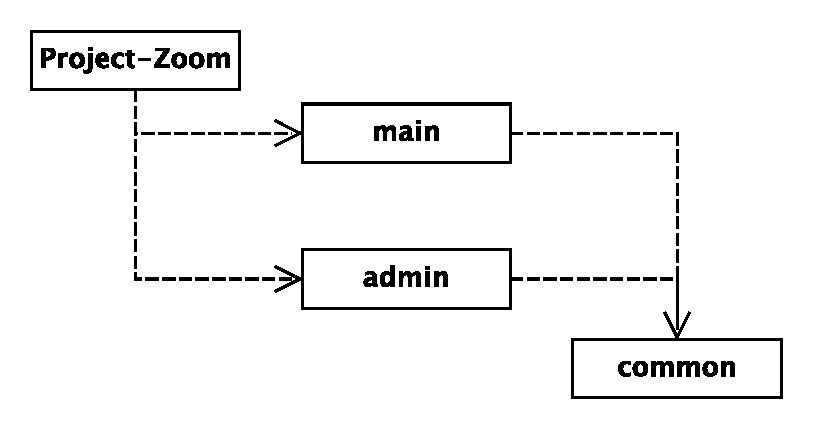
\includegraphics[width=0.8\textwidth]{img/projekte.pdf}  
   \caption{Projekte und deren Abhängigkeiten}   
  \label{fig:projects} 
\end{figure}

\FloatBarrier
In der Abbildung \ref{fig:projects} sind die Abhängigkeiten der Pakete voneinander dargestellt. Das Anlegen eines Hauptprojektes, in diesem Fall Project-Zoom, erleichtert die Arbeit mit dem Gesamtprojekt. Durch die Abhängigkeit zu \tete{main} und \tete{admin} muss nur noch das Hauptprojekt kompiliert werden, denn die Abhängigkeiten werden bei Änderungen im Source-Code automatisch mit kompiliert.

\section{Data-centric Design in Project-Zoom}
\label{sec:umsetzung_dcd}
Die REST-Schnittstelle von Project-Zoom entspricht der einer klassischen CRUD-Anwendung. Aufgrund der geringen Business-Logik liegt es nahe, das beschriebene data-centric Design zu verwenden. Um die Wartung des Systems zu erleichtern, werden Datenzugriffsobjekte für jedes Datenmodell verwendet.
\\\\\\
\lstinputlisting[caption=Macro-Verwendung zur Generierung einer JSON-Konvertierung, label=lst:json-format, language=scala]{code/json_reads.scala}

Für einige Teile der Anwendung ist es notwendig die JSON-Strukturen der Datenbank in Scala-Objekte umzuwandeln. Dies ist zum Beispiel für User-Objekte der Fall, welche von der Authentifizierungsbibliothek SecureSocial verwendet werden. Play erlaubt die Generierung der Transformationsfunktionen mit Hilfe von Macros\footnote{JSON Macro incepetion, \url{http://www.playframework.com/documentation/2.1.1/ScalaJsonInception} (Zugriff 26.06.13)}. Das bedeutet, dass die Anwendung die Datenklassen des Modells definiert und die Funktionen zur Konvertierung von und nach JSON während der Kompilierung vom Framework übernommen werden. Ein Beispiel für solch eine Transformation ist in dem Quelltext \ref{lst:json-format} mit der Variablen \tete{userFormat} gegeben. Diese ist in der Lage, zwischen den beispielhaften Repräsentationen 
\begin{lstlisting} 
{ 
  "firstName" : "Max", 
  "lastName"  : "Mustermann" 
}
\end{lstlisting} und 
\begin{lstlisting} 
User("Max", "Mustermann")
\end{lstlisting} 
zu konvertieren. Die Bedarfskonvertierung ist durch die Verwendung von unveränderbaren Case-Klassen typsicher und entspricht den Konzepten der funktionalen Programmierung (vgl. \cite{functional-thinking}).

Die CRUD-Operationen \tete{list} und \tete{read} wurden implementiert, ohne Datenbankobjekte zu konvertieren. Die Daten werden aus der Datenbank gelesen, transformiert und anschließend an den anfragenden Client zurückgegeben. Bei der Transformation werden z.B. Passwort-Hashes und Login-Informationen, die sich im User-Objekt befinden, entfernt. Die Funktionen \tete{create}, \tete{update} und \tete{delete} sind nicht für alle Datenbankobjekte implementiert. Dies liegt an der Anforderung, dass die Datenhaltung in der von der D-School bereits verwendeten Datenbank geschehen soll. Project-Zoom soll diese Daten nur aggregieren.


\section{Anbindung externer Komponenten}

Die Implementierung des Eventsystems zur Anbindung externer Komponenten in Project-Zoom basiert auf dem Akka-Framework. Die in Absatz \ref{sec:actor} beschriebenen Aktoren eignen sich sehr gut zur Modellierung eines Subscribers. Ein Aktor ist eine abgeschlossene funktionelle Einheit, deren Kommunikation nur über unveränderbare Nachrichten erfolgt. Erhält ein Aktor eine Nachricht, so wird diese in der Mailbox gesammelt. Die Nachrichten in der Mailbox werden dann mit Hilfe der \qc{receive}-Funktion, welche jeder Aktor definieren muss, abgearbeitet. 

In der Umsetzung erfolgt das Abonnieren einer Nachricht durch das Senden einer partiellen Funktion\footnote{Eine partielle Funktion $f: A \rightarrow B$ ist im Gegensatz zu einer totalen Funktion nicht auf jedem Wert aus $A$ definiert. Für die Anwendung in Scala siehe \cite{partial-function}.} an den Dispatcher. Diese Funktion bildet den Typ \tete{Event} auf \tete{Unit}\footnote{Der Rückgabetyp Unit entspricht dem Java Pendant \tete{void}.} ab und ist auf allen Events definiert, welche der Subscriber empfangen will. Der Dispatcher benutzt anschließend alle partiellen Funktionen, um eine eingehende Nachricht zu verteilen. Standardmäßig hat ein Subscriber alle Nachrichten abonniert, für die seine \qc{receive}-Funktion definiert ist.

\subsection{Anbindung der Konnektoren und des Thumbnailgenerators}

Externe Komponenten kommunizieren untereinander und mit dem Core über dieses beschriebene Eventsystem. Ein Beispiel solch einer Kommunikation ist in der Abbildung \ref{fig:eventsystem-bsp} zu sehen. Das Sequenzdiagramm zeigt wie ein Konnektor ein neues Artefakt registriert, welches anschließend vom Core und vom Thumnailsystem verarbeitet wird. Eine Übersicht über alle vom Backend-Core empfangenen und gesendeten Events findet sich im Anhang \ref{event-overiview}.

\begin{figure}[h]  
  \centering     
  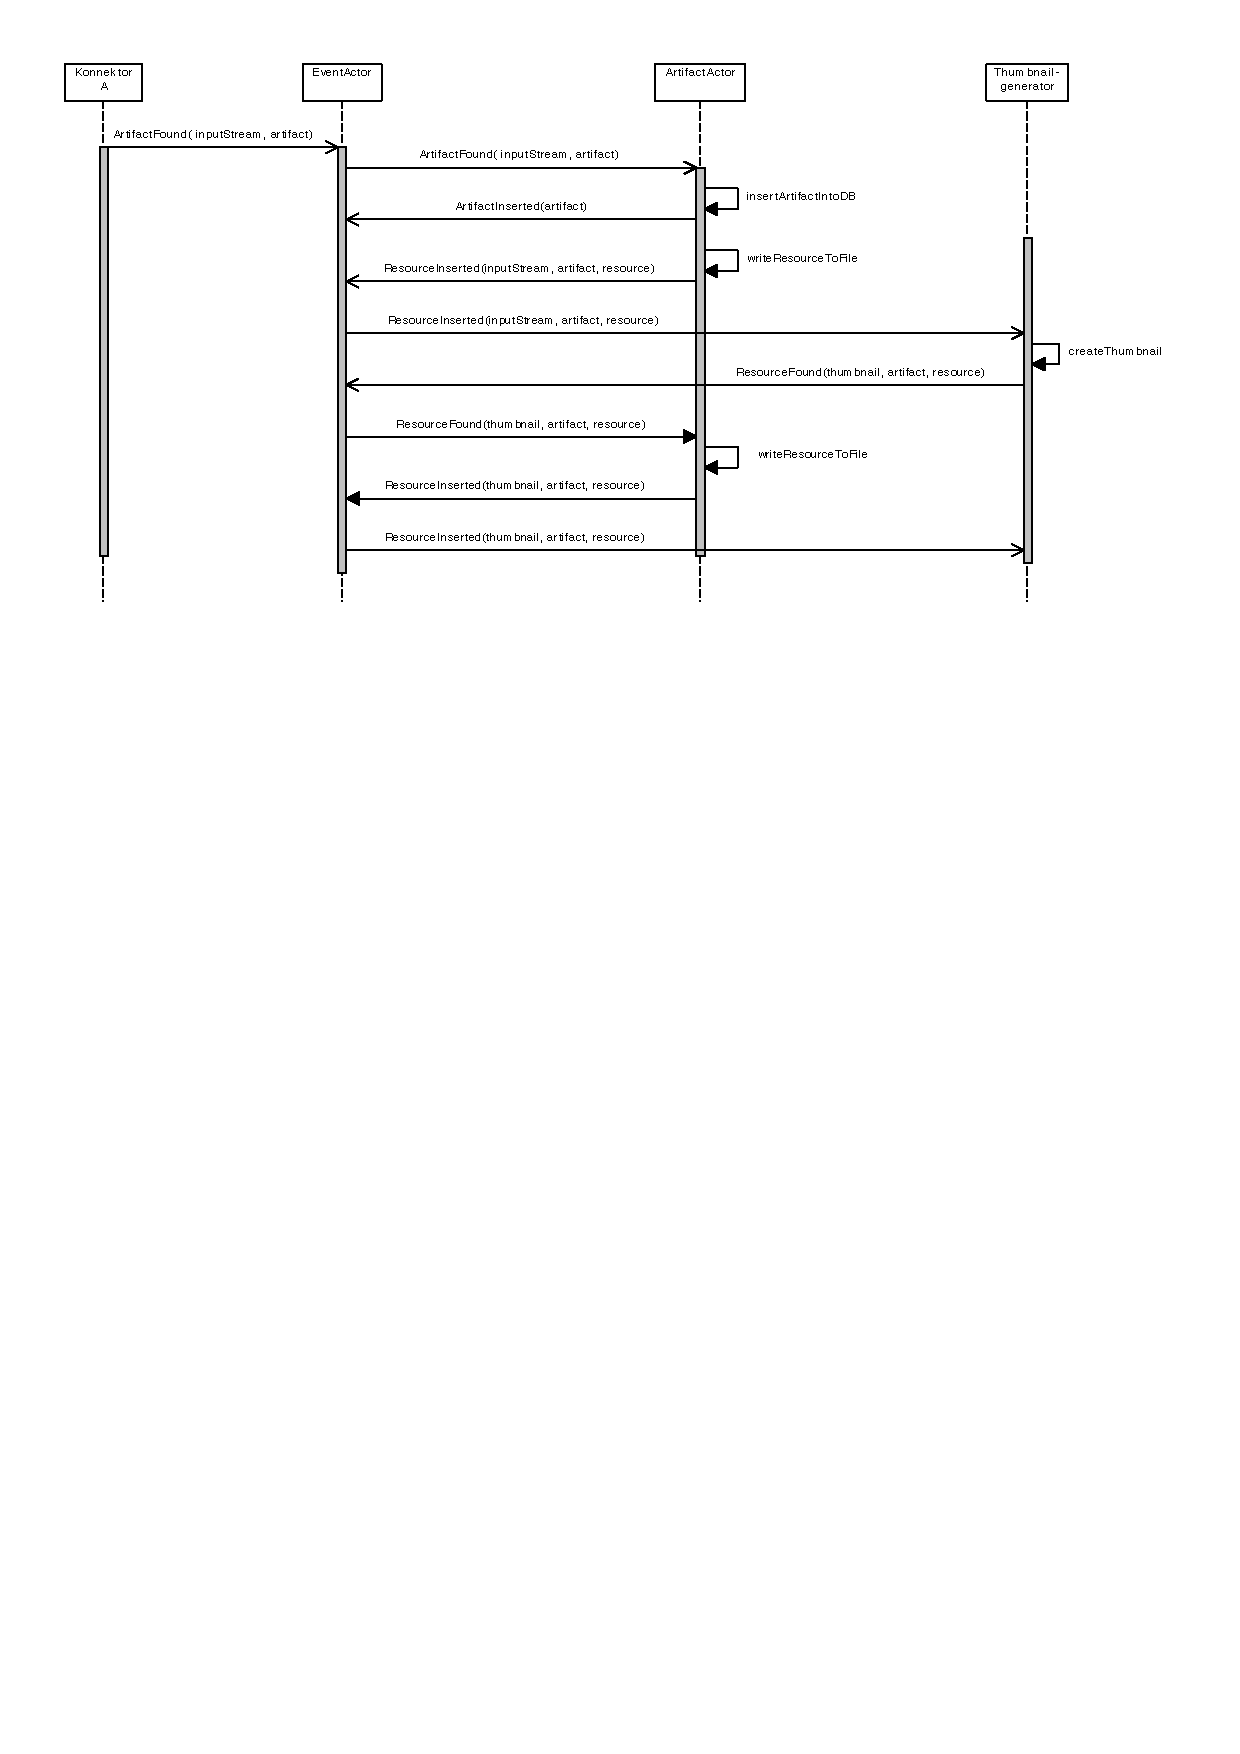
\includegraphics[width=1.0\textwidth]{img/eventsystem_bsp.pdf}  
   \caption{Beispielhafter Ablauf beim Fund eines neuen Artefakts}   
  \label{fig:eventsystem-bsp} 
\end{figure}

\section{Evaluierung der Anforderungen}

Den Abschluss der Betrachtungen zur Implementierung soll ein Rückblick auf die im Abschnitt \ref{sec:requirements} aufgestellten Anforderungen an das System bilden.

Es wurde ein System entwickelt, welches zur Trennung von Administration und Nutzung in Module geteilt ist. Die Webanwendung ist durch das Authentifizierungsmodul SecureSocial und die implementierten Autorisierungsmechanismen in den Datenbankzugriffsobjekten geschützt (vgl. Anforderung \ref{itm:f1}). Die Anwendung ist aus dem Internet erreichbar und somit auch außerhalb der D-School verfügbar (vgl. Anforderung \ref{itm:f6}).

Bei der Umsetzung der Konnektoren (vgl. Anforderung \ref{itm:f2}) sei auf die Arbeit von Thomas Werkmeister \cite{bp-tewe}, in welcher die umgesetzten Konnektoren erläutert sind, verwiesen. Die Datenquellen die in \cite{bp-tewe} beschrieben sind, werden durch die Aggregation nicht verändert (vgl. Anforderung \ref{itm:f5}). Die Anforderung \ref{itm:f3} verlangt, dass keine Daten gelöscht werden. Dies wurde umgangen, indem beim Löschen von Elementen aus einer aggregierten Datenquelle die entsprechenden Artefakte als gelöscht markiert werden.

Die Anforderung \ref{itm:f4} stellt den Anspruch auf eine einfache Anbindbarkeit von neuen Datenquellen. Durch das Eventsystem, welches durch den Backend-Core zur Verfügung gestellt wird, ensteht ein System, welches viel Spielraum für das Anbinden neuer Konnektoren bietet.

Um die maximale Last des Systems zu prüfen, wurde mit Hilfe von \tete{Apache HTTP Bench}\footnote{Apache HTTP Server Benchmarking Tool, \url{http://httpd.apache.org/docs/2.2/programs/ab.html} (Zugriff 29.06.13)} ein Lasttest ausgeführt. Bei diesem Test wurde eine maximale Last von im Durchschnitt 461 Anfragen pro Sekunde ermittelt (vgl. Anforderung \ref{itm:nf1}). Nähere Informationen und Ergebnisse finden sich im Anhang \ref{sec:performance-test}.

Die Aktualisierung der angebundenen Datenquellen erfolgt einmal pro Minute (vgl. \cite{bp-tewe}). Damit ist auch die Anforderung \ref{itm:nf2} erfüllt.
  
 	%!TEX root = ../Bachelorarbeit.tex
\chapter{Fazit und Ausblick}
In dieser Arbeit wurde der konzeptionelle Aufbau des umgesetzten IT-Systems für die HPI School of Design Thinking näher erläutert. Es wurde die Architektur beginnend beim Datenmodell, über das Konzept des Data-centric Designs, bis zur Anbindung von externen Datenquellen dargelegt. Dabei wurden die Anforderungen des Projektpartners einbezogen und am Ende deren Umsetzung evaluiert.

Während der Evaluierung des Systems wurden von den Testenden verschiedene Verbesserungen an der Nutzeroberfläche vorgeschlagen (vgl. \cite{bp-tomh}). Diese gilt es zu Evaluieren und mit den Anforderungen der D-School abzugleichen.

Während der Umsetzung des Projekts sind verschiedene Ideen aufgekommen das System zu erweitern. Ein Beispiel ist der Mehrbenutzerbetrieb, in welchem mehrere Studenten gleichzeitig an unterschiedlichen Rechnern den Graphen eines Projektes ändern. Dem Backend fällt hier die Aufgabe zu, diese Änderungen zusammenzuführen und die einzelnen Nutzer auf dem neusten Stand zu halten.

Die Administration des Systems ist ein weiterer Punkt, dem bei der zukünftigen Entwicklung des Projektes mehr Aufmerksamkeit zukommen sollte. Für das erste Testen unwesentliche Funktionalitäten, wie das Administrieren der Nutzer und Projekte, müssen für den Produktivbetrieb umgesetzt werden. Dabei muss in Zusammenarbeit mit der D-School ein Konzept des Datenaustausches mit der internen Projektverwaltung entwickelt und anschließend die entsprechenden Funktionalitäten im Backend umgesetzt werden.

Der Erfolg und die Akzeptanz des Projektes als Dokumentationsvisualiserer hängt vorrangig von der zukünftigen Entwicklung der Nutzerschnittstelle ab. Das Konzept des System wurde von den Studenten sehr gut aufgenommen. Das Ziel muss es also sein, durch die Fortführung der Analyse der Nutzeranforderungen, den kreativen Ideenaustausch mit den Mitarbeitern und Studierenden der D-School aufrechtzuerhalten und so das Projekt ...?


  %%%%%%%%%%%%%%%%%%%%%%%%%%%%%%%%%%%%%%%%%%%%%%%%%%%%%%%%%%%%%
	%% END CONTENT
	%%%%%%%%%%%%%%%%%%%%%%%%%%%%%%%%%%%%%%%%%%%%%%%%%%%%%%%%%%%%%
  
  %%%%%%%%%%%%%%%%%%%%%%%%%%%%%%%%%%%%%%%%%%%%%%%%%%%%%%%%%%%%%
	%% BIBLIOGRAPHY
	%%%%%%%%%%%%%%%%%%%%%%%%%%%%%%%%%%%%%%%%%%%%%%%%%%%%%%%%%%%%%
	\clearpage
	\bibliographystyle{alpha}
	\bibliography{src/_Literatur}

	%%%%%%%%%%%%%%%%%%%%%%%%%%%%%%%%%%%%%%%%%%%%%%%%%%%%%%%%%%%%%
	%% GLOSSARY
	%%%%%%%%%%%%%%%%%%%%%%%%%%%%%%%%%%%%%%%%%%%%%%%%%%%%%%%%%%%%%
	\printglossary[title=Glossar]

	%%%%%%%%%%%%%%%%%%%%%%%%%%%%%%%%%%%%%%%%%%%%%%%%%%%%%%%%%%%%%
	%% APPENDIX
	%%%%%%%%%%%%%%%%%%%%%%%%%%%%%%%%%%%%%%%%%%%%%%%%%%%%%%%%%%%%%
  \begin{appendix} 
		\clearpage
		\small
    \renewcommand{\thepage}{\thechapter-\arabic{page}}
    %\include{src/Anhang}
    %!TEX root = ../../Bachelorarbeit.tex
\appendixChapter{Quelltexte}
\label{app:anhang}

\section{Quelltext-Beispiel für eine JSON-Transformation und -Validierung}
Im Quelltext \ref{app:jsonbsp} ist die Transformierung und Validierung eines JSON-Objektes gezeigt. Zeilen, welche mit \textsc{//>} beginnen, sind Kommentare und zeigen das Ergebnis der vorhergehenden Anweisung.
\lstinputlisting[caption=Beispiel für Play JSON-Transformation bzw. -Validierung, label=app:jsonbsp, language=scala]{code/json_example.scala}

%--------------------------------------------------------------------------------------------------------------------------------------------
\appendixChapter{Interview Protokolle}

\section{Interview 22.11.2012 - Claudia Nikolai }
\label{sec:interview_nikolai}
Claudia Nikolai ist General Programm Manager der D-School.

\subsection*{Zuständigkeiten}
\label{zustaendigkeiten}

\begin{itemize}
\item inhaltliche Programmgestaltung
\item internationale Kooperation
\item Kontakt zu Kunden
\item Ausbildung der Teacher
\item Teacher (an allen Tagen)
\end{itemize}

\subsection*{Austausch mit anderen Teachern}
\label{austauschmitanderenteachern}

\begin{itemize}
\item Teachermeeting
\item E-Mail (Verteiler, Informationen fuer viele Personen)
\item Dropbox\slash E-mail für Content
\end{itemize}

\subsection*{Incom}
\label{incom}

\begin{itemize}
\item space noch nicht privat\slash sichtbar (kein Austausch von vertraulichen Informationen)
\item zu viele Notifications (liest aber alle)
\item nutzt es um Hinweise an andere Teams zu geben
\item sichtet Material an Tagen, an denen keine D-School ist
\end{itemize}

\subsection*{Wichtig für die Dokumentation}
\label{wichtigfuerdiedokumentation}

\begin{itemize}
\item Wie haben die Studenten Empathie bekommen? (Wie und wann haben sie sich in den User hineinvesetzt?)
\item Zitate
\item Dokumentation der Phasen
\item Welche Methode wurde verwendet und wie gut hat sie funktioniert? -> Evaluierung des DS-Prozesses
\end{itemize}

\subsection*{Wunschsystem}
\label{wunschsystem}

\begin{itemize}
\item System sollte einfach verständlich sein, Nutzer haben nur 6--12 Wochen um damit klar zu kommen
\item System muss keine eierlegende Wollmilchsau sein
\end{itemize}

%--------------------------------------------------------------------------------------------------------------------------------------------
\appendixChapter{Ergänzende Visualisierungen}

\section{Datenmodell von Project-Zoom}
In der Abbildung \ref{fig:complete-model} ist das komplette Datenmodell von Project-Zoom dargestellt.
\begin{figure}[h!t]
  \centering     
  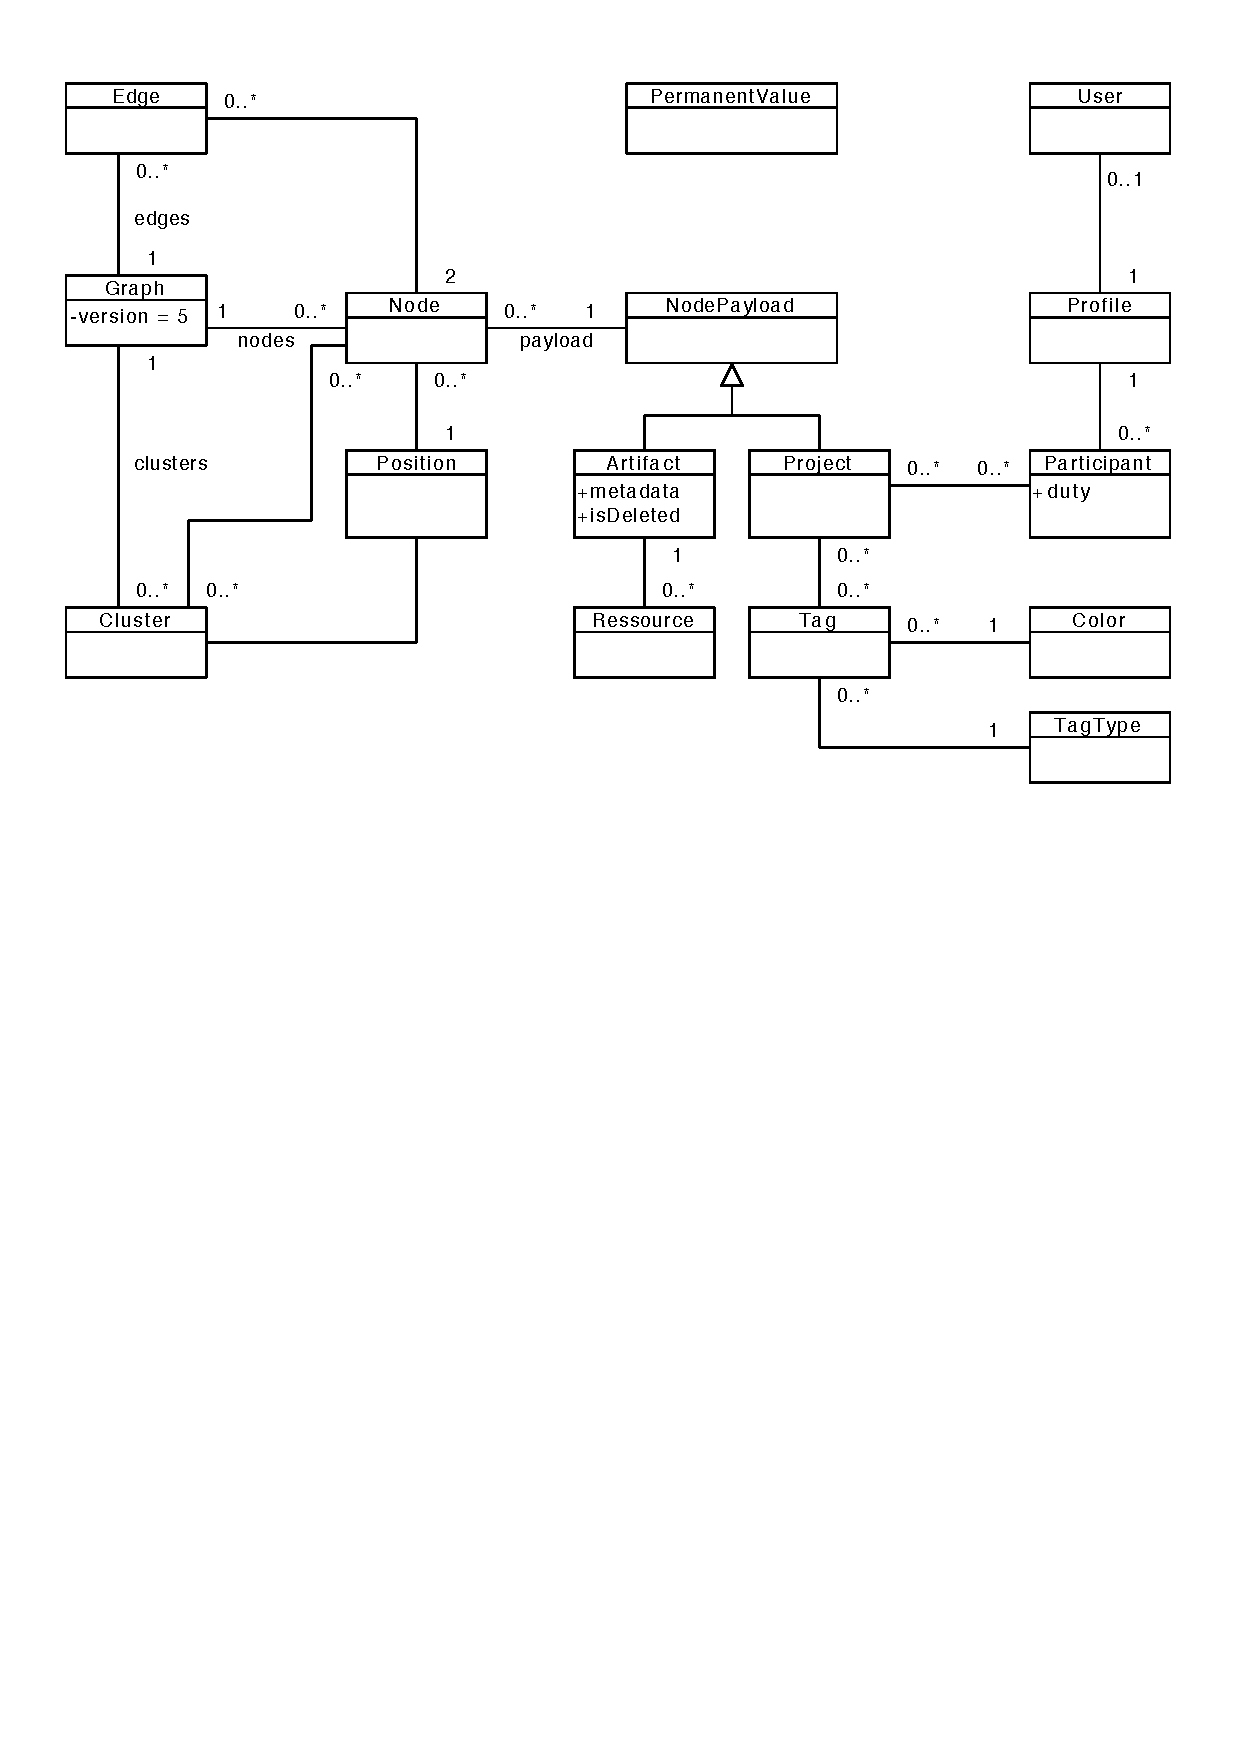
\includegraphics[width=1.0\textwidth]{img/complete_model.pdf}  
   \caption{Datenmodell von Project-Zoom}
  \label{fig:complete-model} 
\end{figure}
\pagebreak
\section{Objektdiagramm für einen beispielhaften Graphen}
\begin{figure}[h!t]
  \centering     
  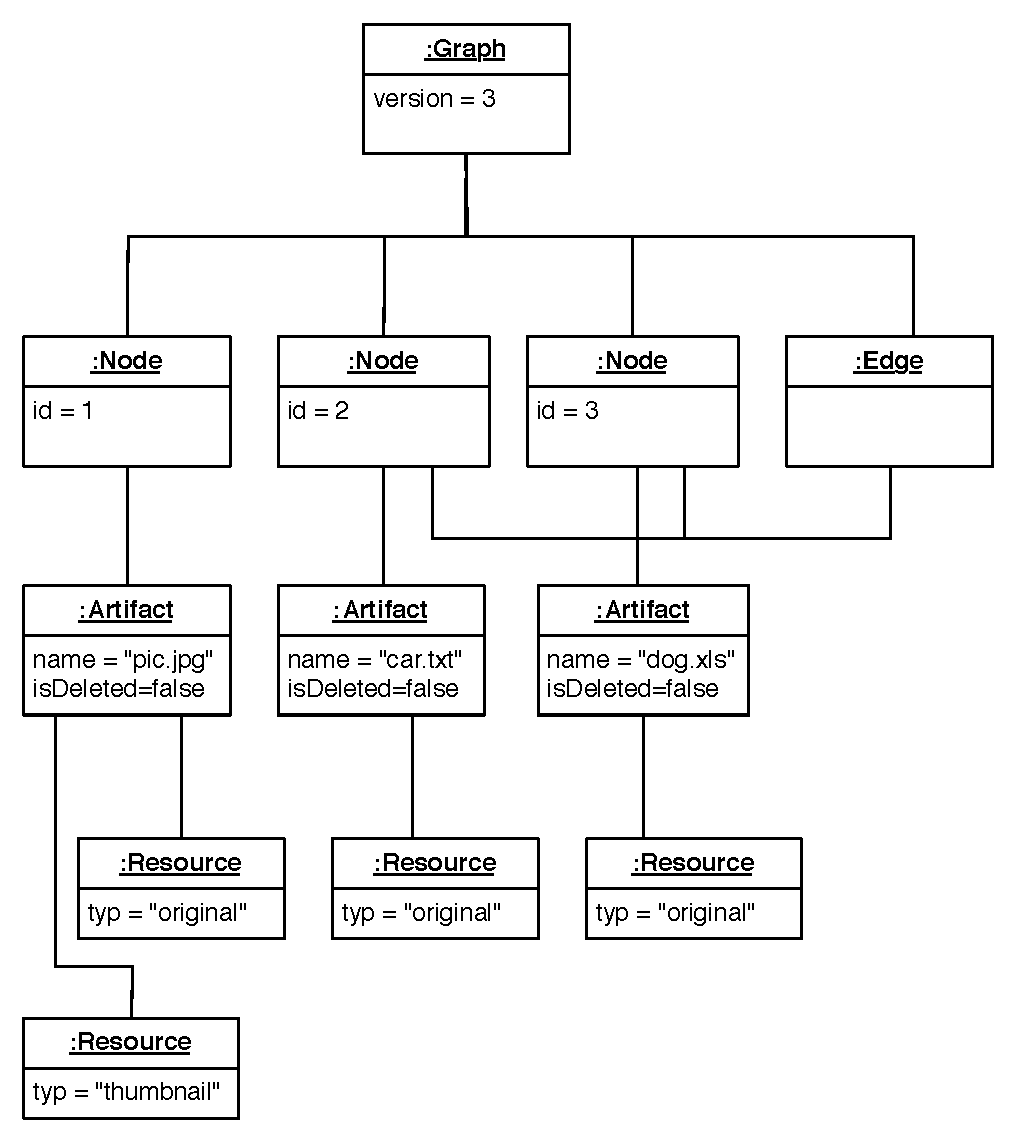
\includegraphics[width=0.8\textwidth]{img/instanz_graph.pdf}  
   \caption{Objektdiagramm eines beispielhaften Graphen. Zur Wahrung der Übersichtlichkeit ist die Position jedes Nodes nicht als Objekt visualisiert.}
  \label{fig:graph-bsp} 
\end{figure}
 
\section{InfoQ Umfrage zu Webframeworks der JVM}
In der Tabelle in der Abbildung \ref{fig:infoq-survey} sind die Umfrageergebnisse der InfoQ-Umfrage mit 1894 Teilnehmern von der Seite \url{http://www.infoq.com/research/jvm-web-frameworks.auf} zum angegebenen Zeitpunkt zu sehen.
\begin{figure}[ht]  
  \centering     
  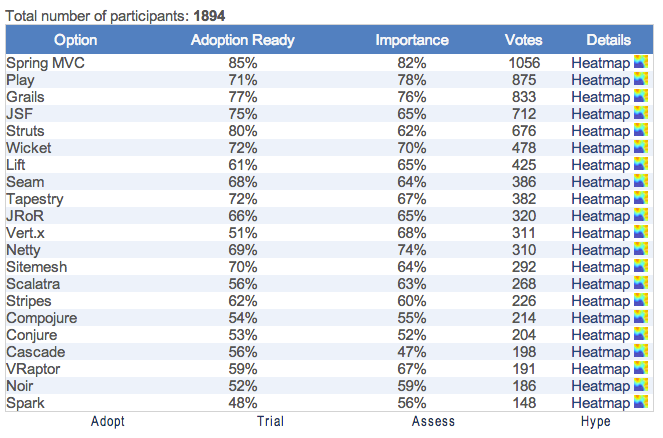
\includegraphics[width=1.0\textwidth]{img/infoq.png}  
   \caption{Stand der Umfrage am 26. Juni 2013}
  \label{fig:infoq-survey} 
\end{figure}

\section{Performance Test}
\label{sec:performance-test}
Project-Zoom wurde mit den folgenden Einstellungen für Apache Bench getestet:
\begin{lstlisting}
ab -g output100.txt -c 10 -n 100000 http://localhost:9000/projects
\end{lstlisting}

Weiterhin wurde noch ein Session-Cookie übergeben, um auf die geschütze Ressource zugreifen zu dürfen. Die Ergebnisse sind in den Abbildungen \ref{fig:perf1} und \ref{fig:perf2} zu sehen. Die Grafiken wurden mit Hilfe von \url{https://loadosophia.org} erstellt.

\begin{figure}
  \centering     
  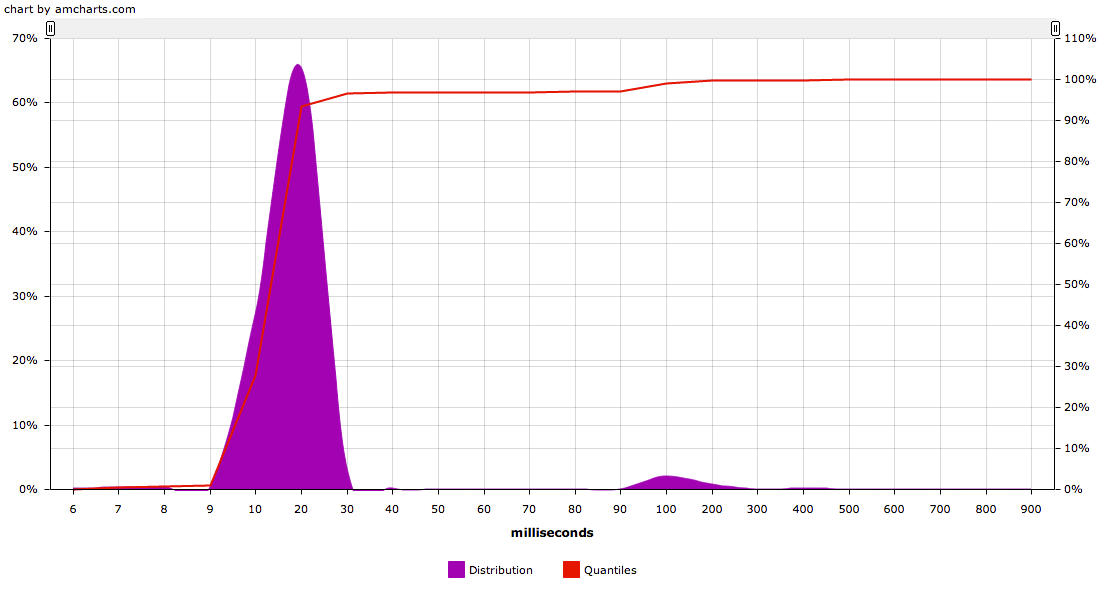
\includegraphics[width=1.0\textwidth]{img/perf1.png}  
   \caption{Dichte- und Verteilungsfunktion der Antwortzeiten }
  \label{fig:perf1} 
\end{figure}

\begin{figure}  
  \centering     
  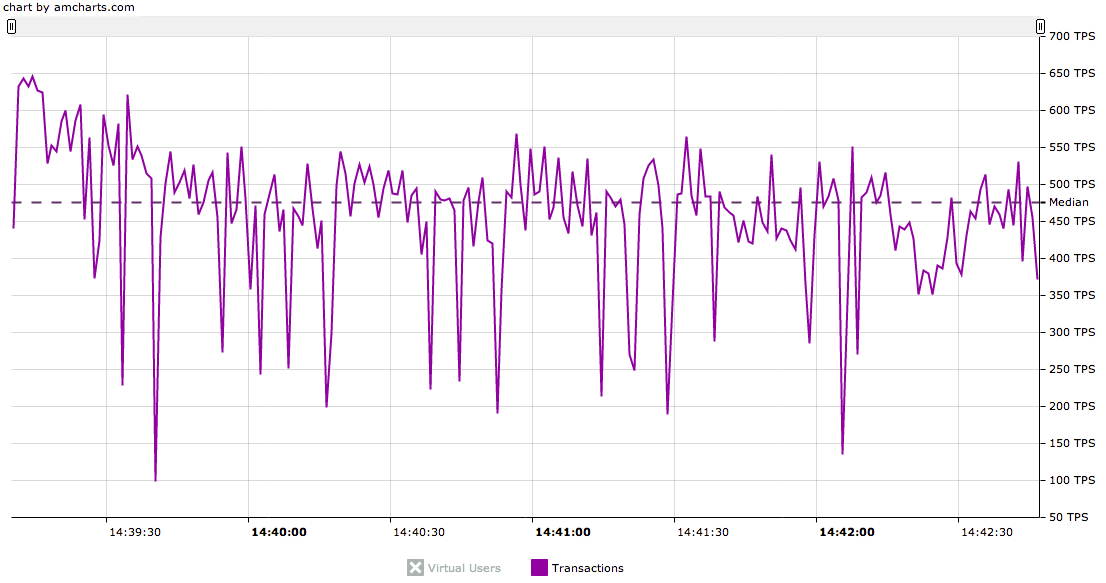
\includegraphics[width=1.0\textwidth]{img/perf2.png}  
   \caption{Durchsatz in abgeschlossenen Übertragungen pro Sekunde über die Zeit}
  \label{fig:perf2} 
\end{figure}


\section{Überblick über die vorhandenen Events}
\label{event-overiview}
In der Tabelle \ref{tab:events} sind alle Events zu sehen, die mit dem Backend-Core interagieren.

\begin{table}
    \begin{tabular}{|l|l|p{4.8cm}|}
    \hline
    ~                   & Parameter                                                                & Bedeutung                                                  \\ \hline
    ArtifactFound       & \begin{lstlisting}[gobble=4] 
    originalStream: InputStream
    artifact: ArtifactLike
    \end{lstlisting}                      & Artefakt von Konnektor gefunden                            \\ \hline
    ArtifactDeleted     & \begin{lstlisting}[gobble=4]
    artifact: ArtifactLike
    \end{lstlisting}                                                   & Löschung von Artefakt durch Konnektor festgestellt         \\ \hline
    ArtifactAggregation & \begin{lstlisting}[gobble=4]
    _project: String
    l: List[ArtifactFound]
    \end{lstlisting}                                 & Auflistung aller Artefakte eines Projektes durch Konnektor \\ \hline
    ArtifactRenamed     & \begin{lstlisting}[gobble=4]
    artifact: ArtifactLike
    name: String
    \end{lstlisting}                                     & Umbenennung von Artefakt durch Konnektor festgestellt      \\ \hline
    ArtifactMoved       & \begin{lstlisting}[gobble=4]
    artifact: ArtifactLike
    path: String
    \end{lstlisting}                                     & Verschiebung von Artefakt durch Konnektor festgestellt     \\ \hline
    ResourceFound       & \begin{lstlisting}[gobble=4]
    inputStream: InputStream
    artifact: ArtifactLike
    resource: ResourceLike
    \end{lstlisting} & Neue Resource für Artefakt gefunden                        \\ \hline
    ArtifactUpdated     & \begin{lstlisting}[gobble=4]
    artifact: ArtifactLike
    \end{lstlisting}                                                   & Artefakt in der DB geändert                                \\ \hline
    ArtifactInserted    & \begin{lstlisting}[gobble=4]
    artifact: ArtifactLike    
    \end{lstlisting}                                               & Artefakt zur DB hinzugefügt                                \\ \hline
    ResourceUpdated     & \begin{lstlisting}[gobble=4]
    file: File
    artifact: ArtifactLike
    resource: ResourceLike
    \end{lstlisting}               & Resource in der DB geändert                                \\ \hline
    ResourceInserted    & \begin{lstlisting}[gobble=4]
    file: File
    artifact: ArtifactLike
    resource: ResourceLike
    \end{lstlisting}               & Resource zur DB hinzugefügt                                \\ \hline
    ProjectFound        & \begin{lstlisting}[gobble=4]
    project: ProjectLike
    \end{lstlisting}                                                     & Projekt von Konnektor gefunden                             \\ \hline
    ProjectAggregation  & \begin{lstlisting}[gobble=4]
    l: List[ProjectFound]      
    \end{lstlisting}                                               & Auflistung mehrerer gefundener Projekte                    \\ \hline
    ProfileFound        & \begin{lstlisting}[gobble=4]
    profile: Profile   
    \end{lstlisting}                                                       & Profil von Konnektor gefunden                              \\ \hline
    ProfileAggregation  & \begin{lstlisting}[gobble=4]
    l: List[ProfileFound]  
    \end{lstlisting}                                                   & Auflistung mehrerer gefundener Profile                     \\ \hline
    GraphUpdated        & \begin{lstlisting}[gobble=4]
    graph: Graph
    patch: JsValue
    \end{lstlisting}                                             & Graph in der DB mit Patch geändert                         \\ \hline
    \end{tabular}
    \caption{Übersicht über Events des Backend-Core}
    \label{tab:events}
\end{table}

\textsc{ArtifactActor}
\begin{labeling}{\textbf{Subscription f{\"u}r:}}
  \item[Publishes] ArtifactUpdated, ArtifactInserted, ResourceUpdated, ResourceInserted
  \item[Subscription f{\"u}r] ArtifactFound, ArtifactDeleted, ArtifactAggregation, ArtifactRenamed, ArtifactMoved, ResourceFound
\end{labeling}

\textsc{KnowledgeActor}
\begin{labeling}{\textbf{Subscription f{\"u}r:}}
  \item[Subscription f{\"u}r] ProjectFound, ProjectAggregation, ProfileFound, ProfileAggregation
\end{labeling}

\textsc{Konnektoren}
\begin{labeling}{\textbf{Subscription f{\"u}r:}}
  \item[Publishes] ProfileAggregation, ProjectAggregation, ArtifactFound, ArtifactRenamed, ArtifactMoved, ArtifactDeleted, ArtifactAggregation
\end{labeling}

\textsc{Thumbnailgenerator}
\begin{labeling}{\textbf{Subscription f{\"u}r:}}
  \item[Publishes] ResourceFound
  \item[Subscription f{\"u}r] ResourceInserted, ResourceUpdated
\end{labeling}

\appendixChapter{REST-Schnittstelle}
\label{sec:rest-interaface}
	\end{appendix}
	
	%%%%%%%%%%%%%%%%%%%%%%%%%%%%%%%%%%%%%%%%%%%%%%%%%%%%%%%%%%%%%
	%% STATURATION DECLARATION
	%%%%%%%%%%%%%%%%%%%%%%%%%%%%%%%%%%%%%%%%%%%%%%%%%%%%%%%%%%%%%
	\chapter*{Eidesstattliche Erkl\"arung}
\clearscrheadfoot

Ich erkl\"are hiermit, dass ich die vorliegende Arbeit selbstst\"andig verfasst und daf\"ur keine
anderen als die genannten Quellen und Hilfsmittel verwendet habe.

\begin{flushleft}
\vspace{3cm}
\docAuthor
\end{flushleft}
\begin{flushleft}
\selectlanguage{german}
\docCity{} \docDate
\end{flushleft}

\end{document}
%%%%%%%%%%%%%%%%%%%%%%%%%%%%%%%%%%%%%%%%%%%%%%%%%%%%%%%%%%%%%
%% END DOKUMENT
%%%%%%%%%%%%%%%%%%%%%%%%%%%%%%%%%%%%%%%%%%%%%%%%%%%%%%%%%%%%%